\documentclass{article}

% if you need to pass options to natbib, use, e.g.:
% \PassOptionsToPackage{numbers, compress}{natbib}
% before loading nips_2016
%
% to avoid loading the natbib package, add option nonatbib:
% \usepackage[nonatbib]{nips_2016}

\usepackage{nips_2016}

% to compile a camera-ready version, add the [final] option, e.g.:
% \usepackage[final]{nips_2016}

\usepackage[utf8]{inputenc} % allow utf-8 input
\usepackage[T1]{fontenc}    % use 8-bit T1 fonts
\usepackage{hyperref}       % hyperlinks
\usepackage{url}            % simple URL typesetting
\usepackage{booktabs}       % professional-quality tables
\usepackage{amsfonts}       % blackboard math symbols
\usepackage{nicefrac}       % compact symbols for 1/2, etc.
\usepackage{microtype}      % microtypography
%\usepackage[english]{babel}
%\usepackage{cite}
%\usepackage{verbatim}
\usepackage{amsmath}
\usepackage{amssymb,amsbsy,epsfig,float}
\usepackage{graphicx,wrapfig,lipsum}
%\usepackage{graphicx}
%\usepackage{multirow}
%\usepackage{algorithmicx}
%\usepackage[ruled]{algorithm}
%\usepackage{algpseudocode}

\usepackage{color}
\usepackage[usenames,dvipsnames]{xcolor}

\usepackage[backgroundcolor = White,textwidth=\marginparwidth]{todonotes}
% To remove todo notes, simply uncomment the following line and comment out the previous one
% \usepackage[disable,backgroundcolor = White,textwidth=\marginparwidth]{todonotes}

% Comments by Csaba:
\newcommand{\todoc}[2][]{\todo[color=Apricot!20,size=\tiny,#1]{Cs: #2}}
% Comments by Manjesh:
\newcommand{\todom}[2][]{\todo[color=Cerulean!20,size=\tiny,#1]{M: #2}}
% Comments by Venkatesh:
\newcommand{\todov}[2][]{\todo[color=Purple!20,size=\tiny,#1]{V: #2}}

\newcommand{\hY}{\hat{Y}}

\usepackage[capitalize]{cleveref}


\newtheorem{thm}{Theorem}
\newtheorem{lemma}{Lemma}
\newtheorem{proposition}{Proposition}
\newtheorem{corol}{Corollary}
\newtheorem{example}{Example}
\newtheorem{condition}{Condition}
\newtheorem{remark}{Remark}
\newtheorem{definition}{Definition}
\newtheorem{assumption}{Assumption}
%\newcommand{\one}[1]{\boldsymbol{1}_{#1}}
%\newcommand{\Prob}[1]{\Pr\{#1\}}
%\newcommand{\EE}[1]{\mathbb{E}[#1]}
%\DeclareMathOperator{\sgn}{sgn}

%\title{Sensor Acquisition with no Feedback}
\title{Unsupervised Sequential Sensor Acquisition}

% The \author macro works with any number of authors. There are two
% commands used to separate the names and addresses of multiple
% authors: \And and \AND.
%
% Using \And between authors leaves it to LaTeX to determine where to
% break the lines. Using \AND forces a line break at that point. So,
% if LaTeX puts 3 of 4 authors names on the first line, and the last
% on the second line, try using \AND instead of \And before the third
% author name.

\author{
	David S.~Hippocampus\thanks{Use footnote for providing further
		information about author (webpage, alternative
		address)---\emph{not} for acknowledging funding agencies.} \\
	Department of Computer Science\\
	Cranberry-Lemon University\\
	Pittsburgh, PA 15213 \\
	\texttt{hippo@cs.cranberry-lemon.edu} \\
	%% examples of more authors
	%% \And
	%% Coauthor \\
	%% Affiliation \\
	%% Address \\
	%% \texttt{email} \\
	%% \AND
	%% Coauthor \\
	%% Affiliation \\
	%% Address \\
	%% \texttt{email} \\
	%% \And
	%% Coauthor \\
	%% Affiliation \\
	%% Address \\
	%% \texttt{email} \\
	%% \And
	%% Coauthor \\
	%% Affiliation \\
	%% Address \\
	%% \texttt{email} \\
}

\begin{document}
	% \nipsfinalcopy is no longer used
	
	\maketitle
	
	\begin{abstract}
		We propose a sensor acquisition problem (SAP) wherein sensors (and sensing tests) are organized into a cascaded architecture and the goal is to choose a test with the optimal cost-accuracy tradeoff for a given instance. We consider the case where we obtain no feedback in terms of rewards for our chosen actions apart from test observations. Absence of feedback raises fundamentally new challenges since one cannot infer potentially optimal tests. We pose the problem in terms of competitive optimality with the goal of minimizing cumulative regret against optimally chosen actions in hindsight. In this context we introduce the notion of weak dominance and show that it is necessary and sufficient for realizing sub-linear regret. Weak dominance on a cascade supposes that a child node in the cascade has higher accuracy when its parent node makes correct predictions. When weak dominance holds we show that we can reduce SAP to a corresponding multi-armed bandit problem with side observations. Empirically we verify that weak dominance holds for many datasets.
	\end{abstract}

\section{Introduction}
%!TEX root =  main.tex
Sequential sensor acquisition arises in many security and healthcare diagnostic systems. In these applications we have a diverse collection of sensor-based-tests with differing costs and accuracy. %Each SBT outputs a prediction of the latent state of an instance.
In these applications (see Fig.~\ref{motiv}) inexpensive tests are first conducted and based on their outcomes a decision for acquiring more (expensive) tests are made. %For instance, in security systems a number of different imaging and non-imaging tests are sequentially processed (see \cite{ML13_MultistageClassifier_TrapezSaligramaCastanon}). Costs can arise due to sensor availability and delay (see Fig.~\ref{motiv}). %A suite of SBTs ranging from inexpensive/rapid tests to more expensive/slow tests are employed. SBTs, as depicted in Fig.~\ref{motiv}, are typically organized in a hierarchical architecture resulting in sequential sensor acquisition of low-cost low-accuracy tests first followed by more expensive higher-accuracy tests. %The task is to determine which tests lead to maximizing accuracy for the available cost-budget. test for clinical diagnosis include genetic markers, imaging (CT, ultrasound, elastography) and biopsy
\begin{figure}[t]
  \centering
  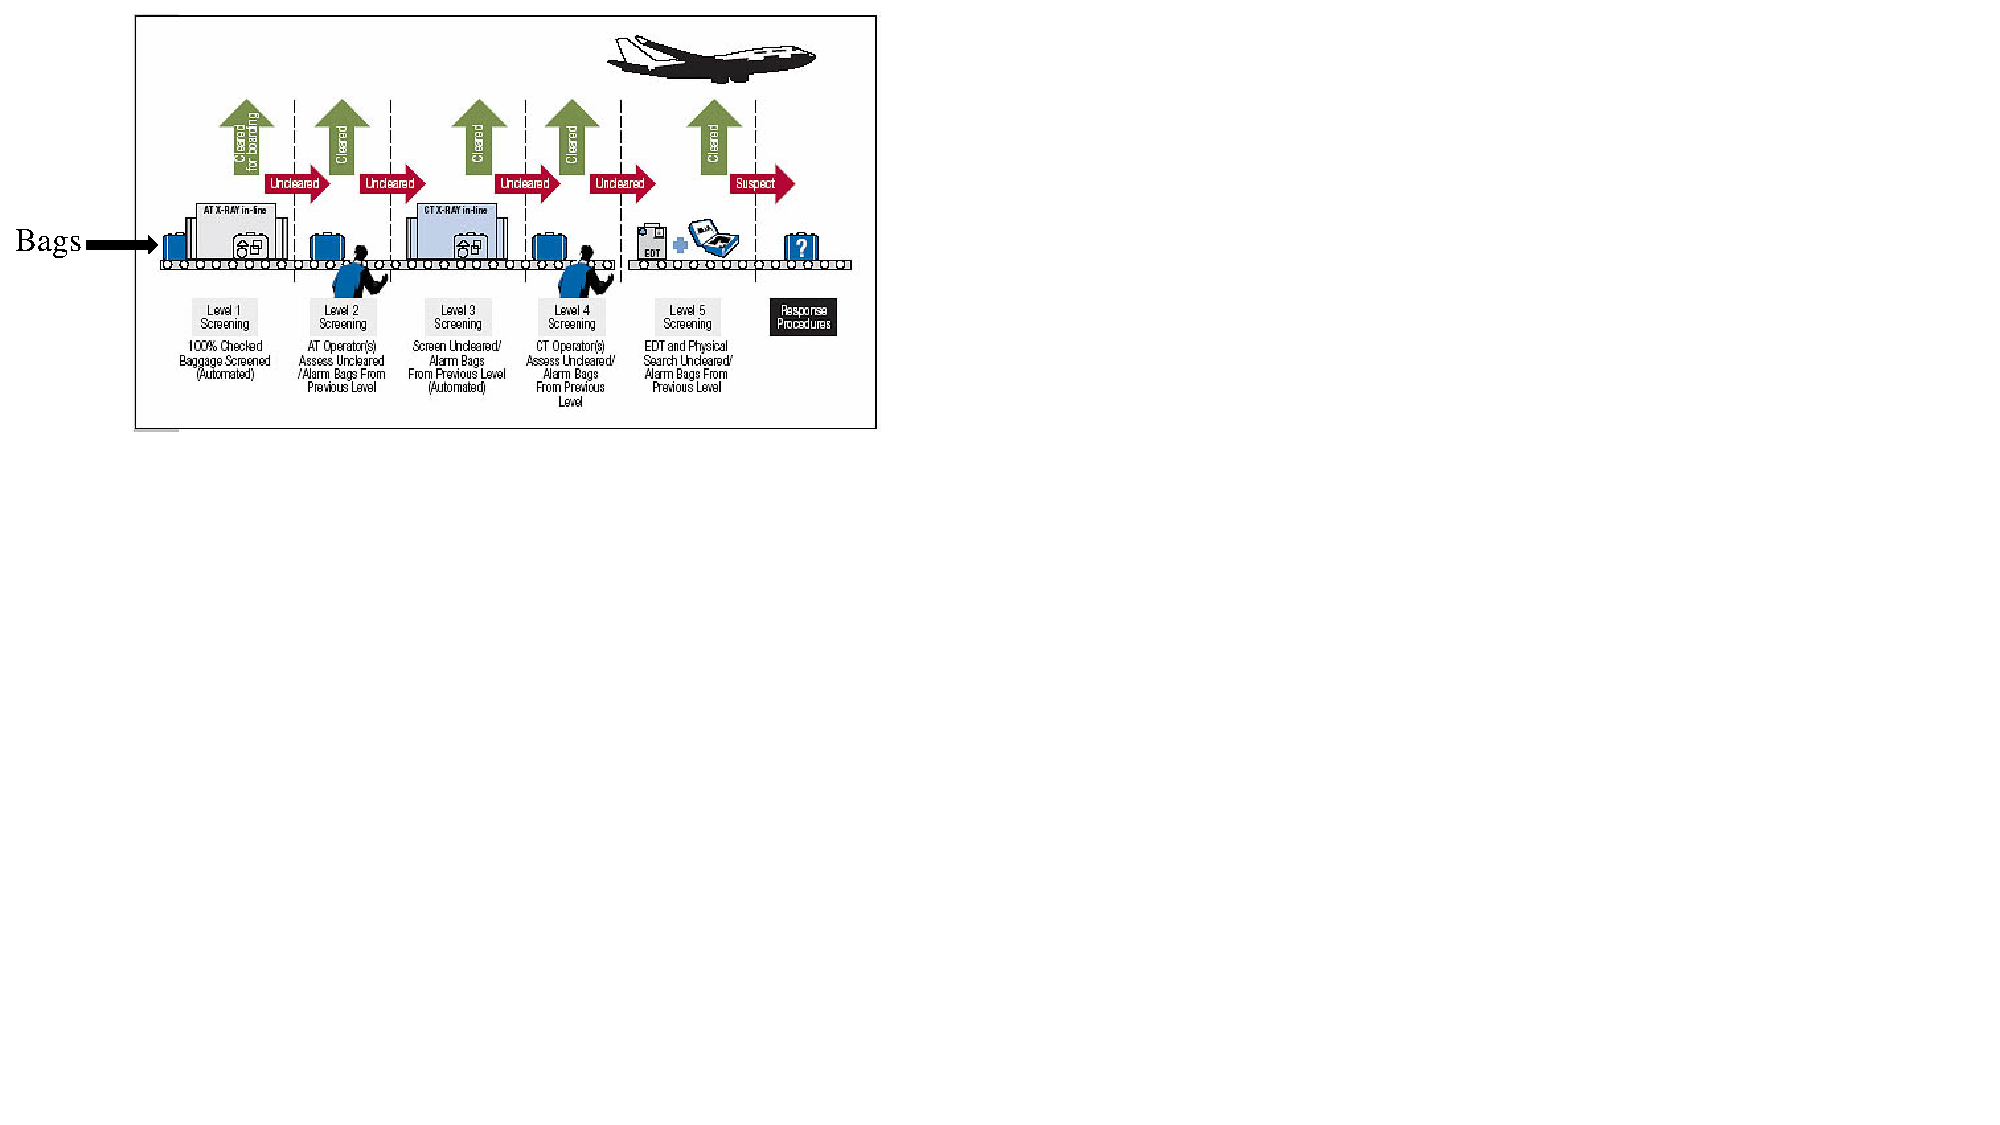
\includegraphics[width=0.4\textwidth]{../Figures/motiv.pdf}
  \caption{\footnotesize Sequential Sensor/Test Selection in Airport Security Systems. A number of different imaging and non-imaging tests are sequentially processed (see \cite{ML13_MultistageClassifier_TrapezSaligramaCastanon}). Costs can arise due to sensor availability and delay. Inexpensive tests are first conducted and based on their outcomes more expensive tests are conducted.}
  \label{motiv}
\vspace{-15pt}
\end{figure}
%Sensor-tests
%Many medical scenraios ranging from chronic diseases to real-time traumatic injury also involve a sequence of tests~\cite{baghdadian}. In the current triaging system the guidelines and standard of care for trauma patients are few and varied. The management of trauma is local and is often managed under institutional, rather than national guidelines~\cite{baghdadian,aastplenary}. In these applications the test 
%
The goal in these systems is to maximize overall accuracy for an available cost-budget. Generally, the components that can be optimized include sensor classifiers (to improve test accuracy), sensor ordering, and decision strategies for sequential sensor selection. Nevertheless, sensor classifiers and sensor ordering are typically part of the infrastructure and generally harder to control/modify in both security and medical systems. To this end we focus here  on the sequential sensor selection problem and use the terms sensor and test interchangeably. The need for systematically learning optimal decision strategies for balancing accuracy \& costs arises from the fact that these applications involve legacy systems where sensor/test selection strategies are local; often managed under institutional, rather than national guidelines~\cite{baghdadian}. %Consequently, systematic techniques for learning optimal decision strategies are required. 
While it is possible to learn such decision strategies given sufficient annotated training data, what makes these applications challenging is that it is often difficult to acquire in-situ ground truth labels. 

These observations motivate the problem of learning decision strategies for optimal sensor selection in situations where we do not have the benefit of ground-truth annotations, and what we refer to as the Unsupervised Sensor Selection (USS) problem. %We assume that the scenario is played over multiple rounds with an instance associated with each round. Each SBT outputs a prediction of the underlying state of the instance (anomaly, threat, disease or nominal etc.) and must be acquired sequentially complying with the cascade architecture in each round. The learner's goal is to figure out the hidden, stochastic state of the instance based on the sensor outputs. Since the learner knows that the sensors are ordered from least to most accurate he/she can use the most accurate sensor among his/her acquired sensors for prediction. Nevertheless, since the learner does not know the sensor accuracy he/she faces the dilemma of as to which sensor to use for predicting this state.
In Sec.~\ref{sec:Setup} we pose our problem as a version of stochastic partial monitoring problem \cite{BaFoPaRaSze14} with \emph{atypical} reward structure, where tests are viewed as actions and sequential observations serves as side information. As is common, we pose the problem in terms of competitive optimality. We consider a competitor who can choose an optimal test with the benefit of hindsight. Our goal is to minimize cummulative regret based on learning the optimal test based on observations in multiple rounds of play. %Stochastic partial monitoring problem is itself a generalization of multi-armed bandit problems, the latter going back to \cite{Tho33}. The availability of predictions of parent sensors of a chosen sensor is viewed as side observation.  
Recall that in a stochastic partial monitoring problem a decision maker needs to choose the action with the lowest expected cost by repeatedly trying the actions and observing some feedback.
The decision maker lacks the knowledge of some key information, such as in our case, the misclassification
error rates of the classifiers, but had this information been available, the decision maker could calculate the
expected costs of all the actions (sensor acquisitions) and could choose the best action (test). The feedback received by the decision maker in a given round depends stochastically on the unknown information and the action chosen.
Bandit problems \cite{Tho33} are a special case of partial monitoring, where the key missing information is the expected
cost for each action, and the feedback is the noisy version of the expected cost of the action chosen.
In the USS problem the learner only observes the outputs of the classifiers, but not the label to be predicted over multiple rounds
in a stochastic, stationary environment. 


%To cast our problem as a partial monitoring problem, \todoc{Do we need this? Or leave this to the reader, just saying that casting our problem as a partial monitoring problem is trivial?} 
%the key unknown information can be the misclassification error rates of the classifiers, an action is identified with 
%the subset of sensors selected, the cost of an action is the sum of the misclassification cost of the classifiers
%that uses the selected sensor subset outputs and the cost of acquiring these sensor outputs,
%while the observed feedback is the vector of predicted labels by each of the classifiers that use 
%the first, the first and second, etc., up to all sensor outputs from the sensors that were selected.
%Note that unlike in a conventional bandit problem, we do not get \emph{direct} 
%feedback of how well our action performed (either noisy or noiseless)\footnote{This problem naturally arises in the surveillance and medical domains. We can perform a battery of tests on an individual in an airport but can never be sure whether or not he/she poses a threat.}.

%Were the probability of error known for each classifier that uses an initial segment of the tests, 
%a decision maker could optimally balance the cost of erroneous decisions and that of the sensor acquisitions'.
%\todoc{This assumes a cost associated with each error; should this be noted?}
%In the learning version of the problem, the misclassification probabilities are \emph{a priori} unknown and a learner must learn the optimal balance based on some feedback available to him. 
%In the \emph{unsupervised} version considered here
%and which we call the unsupervised \emph{sequential sensor acquisition problem} (SAP),
%the learner only observes the outputs of the classifiers, but not the label to be predicted over multiple rounds
%in a stochastic, stationary environment. 

%This leads us to the following question: Can a learner still achieve the optimal balance in this case?  
In Sec.~\ref{sec:Learnability} we first show (unsurprisingly) that no learner can achieve sublinear regret without further assumptions. To this end we propose the notions of weak and strong dominance, which correspond to constraints on joint probability distributions over the latent state and test-outcomes. Strong Dominance (SD) is a property arising in many Engineered systems and says that whenever a test is accurate on an example, a later test in the sequence is almost surely accurate on that example. %(in other words a child SBT cannot make an error when the parent node is accurate). 
Weak Dominance (WD) is a relaxed notion that allows for errors in these predictions. We empirically demonstrate that WD holds by evaluating it on several real datasets. We also show that in a sense WD is fundamental, namely, without this condition there exist problem instances that result in linear regret. On the other hand whenever this condition is satisfied there exist algorithms that lead to sublinear regret. 

%In particular, we reduce the SAP problem to a stochastic multi-armed bandit with side observations, 
%a problem introduced by \citet{MaSh11}.
Our proof of sublinear regret in Sec.~\ref{sec:Equiv} is based on reducing USS to a version of multi-armed bandit problem (MAB) with side-observation. The latter problem has already been shown to have sub-linear regret in the literature. In our reduction, we identify tests as bandit arms. % are identified by the nodes of the cascade. \todoc{Should we introduce cascade formally then above?}
The payoff of an arm is given by marginal losses relative to the root test, and the side observation structure is defined by the feedback graph induced by the directed graph. We then formally show that there is a one-to-one mapping between algorithms for USS and algorithms for MAB with side-observation. In particular, under WD, the regret bounds for MAB with side-observation then imply corresponding regret bounds for USS.

%\noindent
\subsection{Related Work}
%
%Supervised, batch learning, the problem is well studied.
%
In contrast to our USS setup there exists a wide body of literature dealing with sensor acquisition (see\cite{AISTATS13_SupervisedSequentialLearning_TrapezSaligram}). Like us they also deal with cascade models with costs for features/tests but their method is based on training decision strategies with fully supervised data. There are also several methods that work in an online bandit setting and train prediction models with feature costs \cite{SBCA14:BanditsPaid} but again they require true labels as reward-feedback. A somewhat more general version of \cite{SBCA14:BanditsPaid} is developed in \cite{ZBGGySz13:CostlyFeatures} where in addition the learner can choose to acquire true labels for a cost.

%
%However, unlike us these works focus on prediction-time cost/accuracy tradeoffs, which assumes a fully labeled training set for test-time use. %In particular they assume that a fully labeled training dataset is provided for test-time use. 

Our paper bears some similarity with the concept of active classification, which deals with learning stopping policies\cite{poczos2009,ActiveClass-AIJ-s} among a given sequence of tests. Like us these works also consider costs for utilizing tests and the goal is to learn when to stop to make decisions. Nevertheless, unlike our setup the loss associated with the decision is observed in their context. %when a decision is made. 
%
%
%decide when to quit a cascade that leads to better decisions to maximize throughput against error rates. Again full feedback with accuracy of classification is assumed. Our problem is somewhat related to active classification. Nevertheless, while methods as in \cite{ActiveClass-AIJ-s} seek a classifier that decides what tests to take given the results of previous tests to minimize total cost, they also exclusively deal with batch-supervised learning in this context. The same setting is also studied under hard budget constraints in \cite{LCunderBudget-ECML05}.% and its applications in imaging and computer vision systems are explored in  \cite{ADORE-99,isukapalli01efficient-ICJAI}).
% \todoc{I suspect they assume more than this:
% 	In our previous paper we had a sentence that said that
% 	``their model requires knowing a model of the actions in 
% 	advance'' (this would mean knowing the joint probabilities, I think).}
%  \todoc{Actually, much work exists, need to google this}\todom{Added a line about each reference, not sure if we need to include more similar references}
%
%
%The prediction-time learning \cite{SBCA14:BanditsPaid}, the decision maker can opt to pay for additional observations of the costs associated with other arms. Unlike ours this setting is not unsupervised. In
%\cite{ZBGGySz13:CostlyFeatures}, online learning with costly features and labels is studied.
%In each round, learner has to decide which features to observe, where each feature costs some money. The learner can also decide not to observe the label, but the learner always has the option
%to observe the label. Again this setting is not unsupervised.

%Partial monitoring:
Our paper is related to the framework of finite partial monitoring problems\cite{BaFoPaRaSze14}, which deals with how to infer unknown key information and where tests/actions reveal different types of information about the unknown information. In this context 
%applies to the so-called finite problems (unknown ``key information'') is an element of the probability simplex.
\cite{AgTeAn89:pmon} consider special cases where payoff/rewards for a subset of actions are observed. This is further studied as a side-observation problem in \cite{MaSh11} and as graph-structured feedback \cite{COLT15_OnlineLearningWithFeedback_AlonBianchiDekel, NIPS13_FromBanditsToExperts_AlonBianchiGentile,WGySz:NIPS15}). Our work is distinct from these setups because we are unable to observe rewards for our chosen actions or any other actions.
\vspace{-10pt}
%corresponding to chosen actions (whether the chosen action or in terms of side observations 
%\todom{Need to add Yifan's paper, there seems to be few more based on this in ICML'16, AISTATS'16 and NIPS'16}

%The paper is organized as follows: in Section \ref{sec:background} we give a brief background on online learning problems and discuss information structure in these setups. In Section \ref{sec:Setup} we introduce SAP as a general online learning problem where feedback reveals no information on loss/reward of actions. In Sectjon \ref{sec:Learnability} we identify conditions under which optimal action can be learned in SAP. In Section \ref{sec:Equiv} we establish that SAP is regret equivalent to a stochastic multi-armed bandits with side-observations when it satisfies strong dominance property. When this property holds, Section \ref{sec:Algo} gives an algorithm to solve SAP efficiently. We conclude in Section \ref{sec:Conclu} with a discussion on further extensions.  

\section{Unsupervised Sensor Acquisition Problem}
\label{sec:Setup}
%!TEX root =  main.tex
%The sensors are differentiated in terms of their prediction efficiency and cost. 

\todoc[inline]{
On \cref{wrap-fig:1}:
Why is $Y_t$ the input of the first sensor?
	Should $Y_t$ appear on the figure at all?
	Should not each box take $Z_t$ as input?
	Also, perhaps it should be explained that $Z_t$ is not available
	to the learner. The dotted line should have an arrow at the end?
	}


\todoc[inline]{Starting with a specific example would be much better.}
A learner has access to $K\geq 2$ sensors that provide predictions
of an unknown label. \todoc{We agreed with Venkatesh, that in the intro, he will explain that
the classifiers themselves are a kind of intelligent sensors. So the sensors mentioned here
are really the classifiers themselves. ``Intelligent, super-sensors''.
The advantage of talking about sensors only is that we don't really care about what 
goes into the classifiers anyways.
}
 It is assumed that the sensors form a cascade (cf. \cref{wrap-fig:1}),
i.e., they are  \emph{ordered} in terms of their prediction efficiency,
later sensors are more accurate in predicting the unknown label.
However, acquiring the output of later sensor comes at a fixed cost.
The dilemma of the learner is that while he knows the ordering of the sensors,
the accuracies of the sensors are unknown.
The learner's task is to minimize the total prediction cost, which includes
both the cost of acquiring the sensor outputs and the cost incurred due to imperfect
sensor output.
The learner knows the costs, but does not know how efficient the sensors are
and learns only the output of the sensors.
Learning happens in a sequential setting, where in each round the learner can decide
sequentially (within the round) which sensor outputs to observe,
while respecting the ordering of the sensors.
The output of the last sensor selected serves as the prediction for the round.

The formal specification of the learning problem is as follows:
Learning happens sequentially.
In round $t$ ($t=1,2,\dots$), 
the environment generates 
$(Y_t,\hY_t^1,\dots,\hY_t^K)\in \{0,1\}^{K+1}$ from a distribution $P$ unknown to the learner.
\todoc{Do we use anywhere that labels are binary? If not, why not present a general case?}
Here, $Y_t$ is the unknown label to be predicted in round $t$, while $\hY_t^k$ is the output of sensor
$k$, a prediction of $Y_t$.
At the cost of $c_1+ c_2 + \dots + c_k$,
the learner can choose to acquire the outputs of the first $k$ sensors,
where $k\in [K] := \{1,\dots,K\}$. 
\todoc{Now, here we are not talking about acquiring the sensor outputs in a sequential fashion.
Do we need to modify the introduction where we promised that this will happen? 
Can we justify why won't consider the fully sequential case? For simplicity?
In fact, if we did consider the fully sequential case 
then the natural action space would be more complicated:
The actions would be trees, describing the policies of when to continue to acquire new sensors. 
}
Here, $c_i\ge 0$ is the marginal cost of acquiring the output of sensor $i$.
The costs $c := (c_1,\dots,c_K)$ are known to the learner.
Having acquired the output of the first $k$ sensors, the learner predicts the unknown label $Y_t$ using
the output of the last sensor acquired, i.e., using $\hY_t^k$, making the learner incur the loss
\begin{align*}
L_t(k)=\mathbf{1}_{\{\hat{Y}^k_t\neq Y_t\}}+\sum_{j=1}^k c_j\,
\end{align*}
in round $t$.
The feedback of learner for this round is then $H_t(k)=(\hat{Y}^1_t,\ldots,\hat{Y}^k_t)$.
\todoc{Mention contextual case here, or later?}

%Let $\{Z_t, Y_t\}_{{t>0}}$ denote a sequence generated according to an unknown distribution. $Z_t \in\mathcal{C} \subset  \mathcal{R}^d$, where $\mathcal{C}$ is a compact set, denotes a feature vector/context at time $t$ and $Y_t \in \{0,1\}$ its binary label. We denote output/prediction of the $i^{th}$ sensor as $\hat{Y}^i_t$ when its input is $Z_t$. The set of actions available to the learner is $\mathcal{A}=\{1,\ldots, K\}$, where  the action $k \in \mathcal{A}$ indicates acquiring predictions from sensors $1,\ldots, k$ and classifying using the prediction $\hat{Y}^k_t$. 


\begin{wrapfigure}{r}{5cm}
	\vspace{-.5cm}
	\centering
	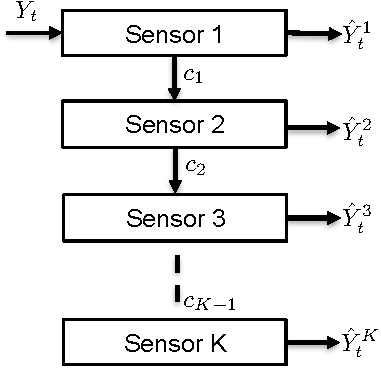
\includegraphics[scale=.6]{SensorCascade.pdf}
	\caption{Cascade of sensors
	}\label{wrap-fig:1}
	\vspace{-.5cm}
\end{wrapfigure} 

\if0
The prediction error rate of the $i^{th}$ sensor is denoted as $\gamma_i:=\Pr\{Y_t\neq \hat{Y}^k_t\}$. The learner incurs an extra cost of $c_k\geq 0$ to acquire output of sensor $k$ after acquiring output of sensor $k-1$. The sensor cascade is depicted in the adjacent figure. In this section we assume that the error rate does not depend on the  context, and the treatment with contextual information is given in the supplementary. 
\fi

%Let $H_t(k)$ denote the feedback observed in round $t$ from action $k$. Since we observe predictions of all the first $k$ senors by playing action $k$, we get   $H_t(k)=(\hat{Y}^1_t,\ldots,\hat{Y}^k_t)$.
%The loss incurred in each round is defined in terms of the prediction error and the total cost involved. When the learner selects action $k$, loss is the prediction error of sensor $k$ plus sum of the costs incurred along the path ($c_1,\ldots,c_k$). Let $L_t: \mathcal{A}\rightarrow \mathcal{R}_+$ denote the loss function in round $t$. Then,
%\begin{equation}
%L_t(k)=\mathbf{1}_{\{\hat{Y}^k_t\neq Y_t\}}+\sum_{j=1}^k c_j.
%\end{equation} 
We refer to the above setup as Sensor Acquisition Problem (SAP).
Based on the previous description, an instance of SAP is the tuple $\psi = (K,P,c)$, where $K\in \mathbb{N}$, $K\ge 2$,
$P$ is a distribution over $\{0,1\}^{K+1}$ and $c\in [0,\infty)^K$. \todoc{I got rid of $c_0$.}
 A policy $\pi$ on a $K$-sensor SAP problem
 is a sequence of maps, $(\pi_1, \pi_2, \cdots)$, where
 $\pi_t : \mathcal{H}_{t-1}\rightarrow [K]$ gives the action selected in round $t$
 given a history $h_{t-1}\in \mathcal{H}_{t-1}$ that consists of all actions and corresponding feedback observed before $t$. 
 Let $\Pi$ denote set of such policies. 
 For any $\pi \in \Pi$, we compare its performance to that of the single best action in hindsight 
 and define its expected regret as follows
\begin{equation}
R^\psi_T(\pi)= \mathbb{E}\left[\sum_{t=1}^T L_t(I_t)\right]-\min_{k\in A}\mathbb{E}\left[\sum_{t=1}^T L_t(k)\right],
\end{equation}
where $I_t$ denotes the action selected by $\pi_t$ in round $t$.
\todoc{I prefer upper case for random variables. Also, later the paper is quite inconsistent in its notation for actions. Sometimes we have $i_s$, $A_t$, then $a_t$, etc. This should be unified.}
The goal of the learner is to learn a policy that minimizes the expected total loss, or, equivalently, to minimize the expected regret, i.e.,
\begin{equation}
\pi^*= \arg \min_{\pi \in \Pi } R^\psi_T(\pi).
\end{equation}

\noindent
{\bf Optimal action in hindsight: } For any $t$, we have 
\begin{equation}
\label{eqn:OptimalAction}
\mathbb{E}[L_t(k)]=\Pr\{Y_t\neq \hat{Y}^k_t\}+\sum_{j=1}^kc_j=\gamma_k +\sum_{j=1}^k c_j\,,
\end{equation}
where $\gamma_k=\Pr\{Y_t\neq \hat{Y}^k_t\}$ is the misclassification error rate of sensor $k$.
Let $k^*=\arg\min_{k\in [K]} \gamma_k + \sum_{i\le  k}c_i$. \todoc{I got rid of $\mathcal{A}$. Let's instead use $[K]$. Simpler. Fewer symbols. Also, for some reason we had $\sum_{i<k}$. I fixed this.}
Then the optimal policy is to play action $k^*$ in each round. 
If an action $i$ is played in any round then it adds $\Delta_k:=\gamma_k + \sum_{i\le k}c_i -( \gamma_{k^*} + \sum_{i\le k^*}c_i)$ to the expected regret. 
Let $I_t$ denote the action selected in round $t$ 
and $N_k(s)$ denote the number of times action $k$ 
is selected till time $s$, i.e., $N_k(s)=\sum_{t=1}^s \boldsymbol{1}_{\{I_t=k\}}$. 
Then the expected regret can be expressed as \todoc{Why do we have this here? Add explanation or remove this.}
\begin{eqnarray}
\label{eqn:ExpRegretGap}
R^\psi_T(\pi)&=& \sum_{k \in \mathcal{A}}\mathbb{E}[N_k(T)]\Delta_k\,.
\end{eqnarray}\



\section{When is SAP Learnable?}
%!TEX root =  main.tex
Let $\TSA$ be the set of all stochastic, cascaded sensor acquisition problems. 
Thus, $\theta \in \TSA$ such that if $Y\sim \theta$ then $\gamma_k(\theta):=\Prob{Y\ne Y^k}$ 
is a decreasing sequence.
Given a subset $\Theta\subset \TSA$, we say that $\Theta$ is \emph{learnable} 
if there exists a learning algorithm $\Alg$ such that
for any $\theta\in \Theta$, the expected regret $\EE{ \Regret_n(\Alg,\theta) }$ 
of algorithm $\Alg$ on instance $\theta$ is sublinear.
A subset $\Theta$ is said to be a maximal learnable problem class if it is learnable and for any $\Theta'\subset \TSA$ superset
of $\Theta$, $\Theta'$ is not learnable.
In this section we study two special learnable problem classes, $\TSD\subset \TWD$, where the regularity properties of the instances in $\TSD$ are more intuitive, while $\TWD$ can be seen as a maximal extension of $\TSD$.

Let us start with some definitions.
Given an instance $\theta \in \TSA$, we can decompose $\theta$ (or $P$) into the joint distribution $P_S$ of the sensor outputs $S = (Y^1,\dots,Y^k)$ and the conditional distribution of the state of the environment, given the sensor outputs, $P_{Y|S}$.
Specifically, letting $(Y,S)\sim P$, for $s\in \{0,1\}^K$ and $y\in \{0,1\}$, $P_S(s) = \Prob{S = s}$ and $P_{Y|S}(y|s) = \Prob{Y=y|S=s}$. We denote this by $P = P_S \otimes P_{Y|S}$.
A learner who observes the output of all sensors for long enough is able to identify 
$P_S$ with arbitrary precision, while $P_{Y|S}$ remains hidden from the learner.
%A problem set $\Theta$ is said to be complete if $\{P_S\,:\, \exists P\in \Theta \text{ s.t. } P = P_S \otimes P_{Y|S} \}=M_1( \{0,1\}^K )$, i.e., all distributions over the sensor outputs are possible under some problem instance in $\Theta$.
 This leads to the following statement:
\begin{prop}
\label{prop:learnablemap}
%Let $\Theta \subset \TSA$ be complete. Then,
A subset $\Theta\subset \TSA$ is learnable 
if and only if there exists a map $a: M_1( \{0,1\}^K )\to [K]$ such that 
for any $\theta \in \Theta$ 
with decomposition $P = P_S \otimes P_{Y|S}$, $a(P_S)$ is an optimal action in $\theta$.
\end{prop}
\begin{proof}
$\Rightarrow$: Let $\Alg$ be an algorithm that achieves sublinear regret
and pick  an instance  $\theta \in\Theta$. Let $P = P_S \otimes P_{Y|S}$.
The regret $\Regret_n(\Alg,\theta)$ of $\Alg$ on instance $\theta$ can be written in the form
\begin{align*}
\Regret_n(\Alg,\theta) = \sum_{k\in [K]} \EEi{P_S}{N_k(n)} \Delta_k(\theta)\,,
\end{align*}
where $N_k(n)$ is the number of times action $k$ is chosen by $\Alg$ during the $n$ rounds while
$\Alg$ interacts with $\theta$, $\Delta_k(\theta) = c(k,\theta) - c^*(\theta)$ is the immediate regret
and $\EEi{P_S}{\cdot}$ denotes the expectation under the distribution induced by $P_S$.
In particular, $N_k(n)$ hides dependence on the iid sequence $Y_1,\dots,Y_n \sim P_S$ 
that we are taking the expectation over here. 
Since the regret is sublinear, for any $k$ suboptimal action, $\EEi{P_S}{N_k(n)} = o(n)$. 
Define $a(P_S) = \min \{ k\in [K]\,;\, \EEi{P_S}{N_k(n)} = \Omega(n) \,\}$. Then, $a$ is well-defined as the distribution of $N_k(n)$ for any $k$ depends only on $P_S$ (and $c$). Furthermore, $a(P_S)$ selects an optimal action.

$\Leftarrow$: Let $a$ be the map in the statement and let $f:\N_+\to\N_+$ be such that $1\le f(n)\le n$ for any  $n\in \N$,
$f(n)/\log(n) \to \infty$ as $n\to \infty$ and $f(n)/n \to 0$ as $n\to \infty$ (say, $f(n) = \lceil \sqrt{n} \rceil$).
Consider the algorithm that chooses $I_t = K$ for the first $f(n)$ steps, after which it estimates $\hat{P}_S$ by
frequency counting and then uses $I_t = a(\hat{P}_S)$ in the remaining $n-f(n)$ trials. 
Pick any $\theta \in \Theta$ so that $\theta = P_S \otimes P_{Y|S}$. 
Note that by Hoeffding's inequality, 
$\sup_{y\in \{0,1\}^K} |\hat{P}_S(y)  - P_S(y)| \le \sqrt{\frac{K\log(4n)}{2f(n)}}$ holds with probability $1-1/n$.
Let $n_0$ be the first index such that for any $n\ge n_0$,
$\sqrt{\frac{K\log(4n)}{2f(n)}}\le \Delta^*(\theta) \doteq \min_{k:\Delta_k(\theta)>0} \Delta_k(\theta)$.
Such an index $n_0$ exists by our assumptions that $f$ grows faster than $n \mapsto \log(n)$.
For $n\ge n_0$, the expected regret of $\Alg$ is at most $n \times 1/n + f(n) (1-1/n) \le 1+f(n) = o(n)$.
\end{proof}

An action selection map  $a: M_1( \{0,1\}^K ) \to [K]$ is said to be \emph{sound} for an instance 
$\theta\in \TSA$ with $\theta = P_S\otimes P_{Y|S}$ if $a(P_S)$ selects an optimal action in $\theta$.
With this terminology, the previous proposition says that a set of instances $\Theta$ is learnable if and only if there exists a
sound action selection map for all the instances in $\Theta$.

A class of sensor acquisition problems that contains instances that satisfy the so-called \emph{strong dominance} condition 
will be shown to be learnable:
\begin{defi}[Strong Dominance]
	An instance $\theta \in \TSA$  is said to satisfy the \emph{strong dominance property} if 
	it holds in the instance that if a sensor predicts correctly
	then all the sensors in the subsequent stages of the cascade also predict correctly, i.e., 
	for any $i\in [K]$,
	\begin{equation}
	\label{eqn:DominanceCondition}
	Y^i=Y \,\, \Rightarrow\,\, Y^{i+1}= \dots =  Y^K = Y
	\end{equation}
	almost surely (a.s.)
	where $(Y,Y^1,\dots,Y^K)\sim P$.
\end{defi}
\begin{table}[h]
\begin{center}
\begin{tabular}[c]{c|c|c|c } 
%	\caption{cap:Error statistics}
dataset & $\gamma_1$ & $\gamma_2$ & $\delta_{12}$\\ \hline \hline
diabetic & $0.288 $ & $ 0.219$  & 0.075\\  \hline
heart & $0.305$ & $0.169$ &  0.051\\  \hline
\end{tabular}
\label{tab:ErrorTable1}
\caption{Error statistics}
\end{center}
\end{table}
Before we develop this concept further we will motivate strong dominance based on experiments on a few real-world datasets. Table \ref{tab:ErrorTable1} lists the error probabilities of the classifiers (sensors) for the heart and diabetic datasets from UCI repository. For both the datasets, $\gamma_1$ denotes the test error of an SVM classifier (linear) trained with low cost features and $\gamma_2$ denotes test error of SVM classifier trained using both low and high-cost features (cf. Section \ref{sec:Experiments}). The last column lists $\delta_{12}:=\Prob{Y^1=Y, Y^2\neq Y}$, the probability that second sensor misclassifies an instance that is correctly classified by the first sensor. Strong dominance is the notion that suggests that this probability is zero. We find in these datasets that $\delta_{12}$ is small thus justifying our notion. In general we have found this behavior is representative of other cost-associated datasets. Note that strong dominance is not merely a consequence of improved accuracy with availability of more features. It is related to better {\it recall rates} of high-cost features relative to low-cost features. %Strong dominance assumption implies that the collection of ''recalled examples'' with low-cost features is a subset of those recalled with high-cost features. 



We next show that strong dominance conditions ensures learnability. To this end,
let $\TSD = \{ \theta\in \TSA\,:\, \theta \text{ satisfies the strong dominance condition } \}$.
%\begin{thm}

%Let $\TSD = \{ \theta\in \TSA\,:\, \theta \text{ satisfies the strong dominance condition } \}$.
\begin{thm}
\label{thm:tsdlearnable}
The set $\TSD$ is learnable.
\end{thm}
We start with a proposition that will be useful beyond the proof of this result.
In this proposition, $\gamma_i = \gamma_i(\theta)$ for $\theta \in \TSA$ and $(Y,Y^1,\dots,Y^K) \sim \theta$.
\begin{prop}\label{prop:gammadiff}
For any $i,j\in [K]$, $\gamma_i - \gamma_j = \Prob{Y^i\ne Y^j} - 2\Prob{ Y^j \ne Y, Y^i=Y}$.
\end{prop}
\begin{proof}

We construct a map as required by~\cref{prop:learnablemap}.
Take an instance $\theta \in \TWD$ and let $\theta = P_S \otimes P_{Y|S}$ be its decomposition
as defined above.
Let $\gamma_i = \Prob{Y^i \ne Y}$, $(Y,Y^1,\dots,Y^K)\sim \theta$.
For identifying an optimal action in $\theta$, it clearly suffices
to know the sign of $\gamma_i + C_i - (\gamma_j +C_j)$ for all pairs $i,j\in [K]^2$.
Since $C_i - C_j$ is known, it remains to study $\gamma_i-\gamma_j$.
Without loss of generality (WLOG) let $i<j$.
Then, 
\begin{align*}
\MoveEqLeft 0  \le \gamma_i  - \gamma_j = \Prob{Y^i\ne Y} - \Prob{Y^j\ne Y} \\
& = \cancel{\Prob{Y^i\ne Y, Y^i=Y^j}} + \Prob{ Y^i\ne Y, Y^i\ne Y^j } - \\
& - \left\{ 
       \cancel{\Prob{Y^j\ne Y, Y^i=Y^j}} + \Prob{ Y^j\ne Y, Y^i\ne Y^j }\right\}\\
& = \Prob{ Y^i\ne Y, Y^i \ne Y^j } + \Prob{Y^i=Y,Y^i\ne Y^j}       \\
& - \left\{ 
	  \Prob{ Y^j \ne Y, Y^i\ne Y^j } + \Prob{ Y^i=Y,Y^i\ne Y^j}
	 \right\}\\
& \stackrel{\footnotesize (a)}{=} \Prob{ Y^j \ne Y^i } -2 \Prob{ Y^j\ne Y, Y^i = Y }\,,
\end{align*}
where in $(a)$ we used that $\Prob{ Y^j \ne Y, Y^i\ne Y^j } =  \Prob{ Y^j\ne Y,Y^i= Y}$ and also
$\Prob{ Y^i=Y,Y^i\ne Y^j} = \Prob{ Y^j\ne Y,Y^i= Y}$
which hold because $Y,Y^i,Y^j$ only take on two possible values.
\end{proof}
\begin{proof}[Proof of \cref{thm:tsdlearnable}]
We construct a map as required by~\cref{prop:learnablemap}.
Take an instance $\theta \in \TSD$ and let $\theta = P_S \otimes P_{Y|S}$ be its decomposition as before.
Let $\gamma_i = \Prob{Y^i \ne Y}$, $(Y,Y^1,\dots,Y^K)\sim \theta$, $C_i = c_1+\dots+c_i$.
For identifying an optimal action in $\theta$, it clearly suffices
to know the sign of $\gamma_i + C_i - (\gamma_j +C_j) = \gamma_i-\gamma_j + (C_i-C_j)$ for all pairs $i,j\in [K]^2$.
Without loss of generality (WLOG) let $i<j$. By \cref{prop:gammadiff},
$\gamma_i - \gamma_j = \Prob{ Y^i \ne Y^j } -2 \Prob{ Y^j\ne Y, Y^i = Y }$.
Now, since $\theta$ satisfies the strong dominance condition, $ \Prob{ Y^j\ne Y, Y^i = Y } = 0$.
Thus, $\gamma_i - \gamma_j = \Prob{ Y^i \ne Y^j }$
which is a function of $P_S$ only.
Since $(C_i)_i$ are known, a map as required by~\cref{prop:learnablemap} exists.
\end{proof}
The proof motivates the definition of weak dominance, a concept that we develop next through a series of smaller
propositions. In these propositions, as before $(Y,Y^1,\dots,Y^K) \sim P$ where $P\in M_1(\{0,1\}^{K+1})$,
 $\gamma_i = \Prob{Y^i \ne Y}$, $i\in [K]$, and $C_i = c_1 + \cdots + c_i$.
We start with a corollary of \cref{prop:gammadiff}
\begin{cor}
\label{cor:gammadiff}
Let $i<j$. Then $0\le \gamma_i -\gamma_j \le \Prob{Y^i\ne Y^j}$.
\end{cor}
\begin{prop}
\label{prop:ilej}
Let $i<j$. Assume 
\begin{align}
\label{eq:cond1}
C_j - C_i \not\in [\gamma_i - \gamma_j, \Prob{Y^i\ne Y^j} )\,.
\end{align}
Then $\gamma_i + C_i \le \gamma_j + C_j$ if and only if $C_j - C_i \ge \Prob{Y^i\ne Y^j}$.
\end{prop}
\begin{proof}
\noindent $\Rightarrow$: From the premise, it follows that $C_j - C_i \ge \gamma_i - \gamma_j$.
Thus, by~\eqref{eq:cond1}, $C_j - C_i \ge \Prob{Y^i\ne Y^j}$.
\noindent $\Leftarrow$: We have $C_j - C_i \ge \Prob{Y^i \ne Y^j} \ge \gamma_i -\gamma_j$, where the last
inequality is by \cref{cor:gammadiff}.
\end{proof}
\begin{prop}
\label{prop:jlei}
Let $j<i$. Assume
\begin{align}
\label{eq:cond2}
C_i - C_j \not\in (\gamma_j - \gamma_i, \Prob{Y^i \ne Y^j} ]\,.
\end{align}
Then, $\gamma_i + C_i \le \gamma_j + C_j$ if and only if $C_i - C_j \le \Prob{Y^i \ne Y^j}$.
\end{prop}
\begin{proof}
\noindent $\Rightarrow$: The condition $\gamma_i + C_i \le \gamma_j + C_j$ implies that $\gamma_j -\gamma_i \ge C_i - C_j$.
By \cref{cor:gammadiff} we get $\Prob{Y^i \ne Y^j} \ge C_i - C_j$.
\noindent $\Leftarrow$: Let $C_i - C_j \le \Prob{Y^i \ne Y^j}$. Then, by \eqref{eq:cond2}, $C_i - C_j \le \gamma_j - \gamma_i$.
\end{proof}
These results motivate the following definition:
\begin{defi}[Weak Dominance]
	An instance $\theta \in \TSA$  is said to satisfy the \emph{weak dominance property} if 
	for $i = a^*(\theta)$,
	\begin{align}
	\label{eq:wd} \forall j>i\,\,: \,\, C_j - C_i \ge \Prob{Y^i\ne Y^j}\,.
	\end{align}
We denote the set of all instances in $\TSA$ that satisfies this condition by $\TWD$.	
\end{defi}
Note that $\TSD\subset \TWD$ since for any $\theta\in \TSD$, any $j>i = a^*(\theta)$, on the one hand $C_j - C_i \ge \gamma_i - \gamma_j$, while on the other hand, by the strong dominance property, $\Prob{Y^i\ne Y^j} = \gamma_i - \gamma_j$.

We now relate weak dominance to the optimality condition described in Eq.~\eqref{eqn:interp_opt}. Weak dominance can be viewed as a more stringent condition for optimal actions. Namely, for an action to be optimal we also require that the marginal cost be larger than marginal \emph{absolute} error:
\begin{equation} \label{eqn:interp_WD}
\underbrace{C_j - C_i}_{\text{Marginal Cost}} \geq \underbrace{ E \left [ \left | \ind{Y_t \ne Y_t^i} - \ind{Y_t \ne Y_t^j} \right | \right ]}_{\text{Marginal Absolute Error}},\,\,\, \forall \, j \geq i\,.
\end{equation}
The difference between marginal error in Eq.~\eqref{eqn:interp_opt} and marginal absolute error is the presence of the absolute value. We will show later that weak-dominant set is a maximal learnable set, namely, the set cannot be expanded while ensuring learnability.


We propose the following action selector $\awd: M_1(\{0,1\}^K)  \to [K]$:
\begin{defi}\label{def:awd}
For $P_S \in M_1(\{0,1\}^K) $ let $\awd(P_S)$ denote the smallest index $i\in [K]$ such that
\begin{subequations}
\begin{align}
\forall j<i \,\,:\,\, C_i - C_j < \Prob{ Y^i \ne Y^j }\,, \label{eq:wd1}\\ 
\forall j>i \,\,:\,\, C_j - C_i \ge \Prob{ Y^i \ne Y^j }\,, \label{eq:wd2}
\end{align}
\end{subequations}
where $C_i = c_1+\cdots + c_i$, $i\in [K]$ and $(Y^1,\dots,Y^K) \sim P_S$.
(If no such index exists, $\awd$ is undefined, i.e., $\awd$ is a partial function.)
\end{defi}
\begin{prop}
\label{prop:awdwelldef}
For any $\theta \in \TWD$ with $\theta = P_S\otimes P_{Y|S}$, $\awd(P_S)$ is well-defined.
\end{prop}
\begin{proof}
Let $\theta\in \TWD$, $i = a^*(\theta)$. Obviously, \eqref{eq:wd2} holds by the definition of $\TWD$.
Thus, the only question is whether \eqref{eq:wd1} also holds.
We prove this by contradiction:
Thus, assume that \eqref{eq:wd1} does not hold, i.e., for some $j<i$, $C_i-C_j \ge \Prob{Y^i \ne Y^j}$. Then, by \cref{cor:gammadiff}, $\Prob{ Y^i \ne Y^j} \ge \gamma_j - \gamma_i$, hence $\gamma_j + C_j \le \gamma_i + C_i$, which contradicts the definition of $i$, thus finishing the proof.
\end{proof}
\begin{prop}
\label{prop:awdsound}
The map $\awd$ is sound over $\TWD$: In particular, for any
$\theta\in \TWD$ with $\theta = P_S\otimes P_{Y|S}$, $\awd(P_S)= a^*(\theta)$.
\end{prop}
\begin{proof}
Take any $\theta\in \TWD$ with $\theta = P_S\otimes P_{Y|S}$, $i = \awd(P_S)$, $j = a^*(\theta)$.
If $i=j$, there is nothing to be proven. Hence, first assume that $j>i$. Then, by~\eqref{eq:wd2}, $C_j - C_i \ge \Prob{Y^i \ne Y^j}$.
By \cref{cor:gammadiff}, $\Prob{Y^i \ne Y^j } \ge \gamma_i - \gamma_j$. Combining these two inequalities we get that
$\gamma_i + C_i \le \gamma_j + C_j$, which contradicts with the definition of $j$.
Now, assume that $j<i$. Then, by~\eqref{eq:wd}, $C_i - C_j \ge \Prob{Y^i \ne Y^j}$.
However, by~\eqref{eq:wd1}, $C_i -C_j < \Prob{Y^i \ne Y^j}$, thus $j<i$ cannot hold either and we must have $i=j$.
\end{proof}
\begin{cor}\label{cor:twdlearnable}
The set $\TWD$ is learnable.
\end{cor}
\begin{proof}
By \cref{prop:awdwelldef}, $\awd$ is well-defined over $\TWD$, while by \cref{prop:awdsound}, $\awd$ is sound over $\TWD$.
By \cref{prop:learnablemap}, $\TWD$ is learnable, as witnessed by $\awd$. \todoc{We should add definitions for these concepts..
namely, $\awd$ well-defined over $\TWD$, $\awd$ sound over $\TWD$, etc.}\todom[]{Csaba, you did this already!!}
\end{proof}
\begin{prop}
\label{prop:awdcorrectimplieswd}
Let $\theta \in \TSA$ and $\theta = P_S\otimes P_{Y|S}$ be such that $\awd$ is defined for $P_S$
and $\awd(P_S) = a^*(\theta)$. Then $\theta \in \TWD$.
\end{prop}
\begin{proof}
Immediate from the definitions.
\end{proof}
An immediate corollary of the previous proposition is as follows:
\begin{cor}\label{cor:awdoutsideincorrect}
Let $\theta \in \TSA$ and $\theta = P_S \otimes P_{Y|S}$. 
Assume that $\awd$ is defined for $P_S$ and $\theta \not\in \TWD$. Then $\awd(P_S) \ne a^*(\theta)$.
\end{cor}
The next proposition states that $\awd$ is essentially the only sound action selector map defined for
 all instances derived from instances of $\TWD$:
\begin{prop}\label{prop:awdunique}
Take any action selector map $a: M_1( \{0,1\}^K ) \to [K]$ which is sound over $\TWD$.
Then, for any $P_S$ such that $\theta = P_S\otimes P_{Y|S}\in \TWD$ with some $P_{Y|S}$,
 $a(P_S) = \awd(P_S)$.
\end{prop}
\begin{proof}
Pick any $\theta = P_S\otimes P_{Y|S}\in \TWD$. If $A^*(\theta)$ is a singleton, then clearly $a(P_S) = \awd(P_S)$ since both are sound over $\TWD$.
Hence, assume that $A^*(\theta)$ is not a singleton.
Let $i = a^*(\theta) = \min A^*(\theta)$ and let $j = \min A^*(\theta) \setminus \{ i \}$.
We argue that $P_{Y|S}$ can be changed so that on the new instance $i$ is still an optimal action, while
$j$ is not an optimal action, while the new instance $\theta' = P_S \otimes P_{Y|S}'$ is in $\TWD$.

The modification is as follows:
Consider any $y^{-j} \doteq (y^1,\dots,y^{j-1},y^{j+1},\dots,y^K)\in \{0,1\}^{K-1}$.
For $y,y^j\in \{0,1\}$, define 
$q(y|y^j) = P_{Y|S}(y|y^1, \dots, y^{j-1}, y^j, y^{j+1},\dots, y^K)$
and similarly let
$q'(y|y^j) = P_{Y|S}'(y|y^1, \dots, y^{j-1}, y^j, y^{j+1},\dots, y^K)$
Then, we let $q'(0|0) = 0$ and $q'(0|1) = q(0|0) + q(0|1)$,
while we let  $q'(1|1) = 0$ and $q'(1|0) = q(1|1) + q(1|0)$.
This makes $P_{Y|S}'$ well-defined ($P_{Y|S}'(\cdot|y^1,\dots,y^K)$ is a distribution for any $y^1,\dots,y^K$).
Further, we claim that the transformation has the property that 
it leaves $\gamma_p$ unchanged for $p\ne j$, while $\gamma_j$ is guaranteed to decrease.
To see why $\gamma_p$ is left unchanged for $p\ne j$ note that
$\gamma_p = \sum_{y^p}  P_{Y^p}(y^p) P_{Y|Y^p}(1-y^p|y^p)$.
Clearly, $P_{Y^p}$ is left unchanged.
Introducing $y^{-k}$ to denote a tuple where the $k$th component is left out,
$P_{Y|Y^p}(1-y^p|y^p) = \sum_{y^{-p,-j}} P_{Y|Y^1,\dots,Y^K}( 1-y^p | y^1,\dots, y^{j-1}, 0, y^{j+1}, \dots, y^K )
+P_{Y|Y^1,\dots,Y^K}( 1-y^p | y^1,\dots, y^{j-1}, 1, y^{j+1}, \dots, y^K )$
and by definition,
\begin{align*}
\MoveEqLeft P_{Y|Y^1,\dots,Y^K}( 1-y^p | y^1,\dots, y^{j-1}, 0, y^{j+1}, \dots, y^K )\\
&\quad +P_{Y|Y^1,\dots,Y^K}( 1-y^p | y^1,\dots, y^{j-1}, 1, y^{j+1}, \dots, y^K )\\
&
=
P_{Y|Y^1,\dots,Y^K}'( 1-y^p | y^1,\dots, y^{j-1}, 0, y^{j+1}, \dots, y^K )\\
&\quad+P_{Y|Y^1,\dots,Y^K}'( 1-y^p | y^1,\dots, y^{j-1}, 1, y^{j+1}, \dots, y^K )\,,
\end{align*}
where the equality holds because ``$q'(y|0)+q'(y|1) = q(y|0) + q(y|1)$''.
Thus, $P_{Y|Y^p}(1-y^p|y^p) = P_{Y|Y^p}'(1-y^p|y^p)$ as claimed.
That $\gamma_j$ is non-increasing follows with an analogue calculation.
In fact, this shows that $\gamma_j$ is strictly decreased
if for any $(y^1,\dots,y^{j-1},y^{j+1},\dots,y^K)\in \{0,1\}^{K-1}$, either $q(0|0)$ or $q(1|1)$ was positive.
If these are never positive, this means that $\gamma_j=1$. 
But then $j$ cannot be optimal since $c_j>0$.
Since $j$ was optimal, $\gamma_j$ is guaranteed to decrease.

Finally, it is clear that the new instance is still in $\TWD$ since  $a^*(\theta)$ is left unchanged.
\end{proof}
The next result shows that
the set $\TWD$ is essentially a maximal learnable set in $\mathrm{dom}(\awd)$:
\begin{thm}
Let $a: M_1(\{0,1\}^K) \to [K]$ be an action selector map
such that $a$ is sound over the instances of $\TWD$.
Then there is no instance $\theta = P_S\otimes P_{Y|S} \in \TSA\setminus \TWD$ such that 
$P_S\in \mathrm{dom}(\awd)$, the optimal action of $\theta$ is unique
\todoc{It would be nice to remove this uniqueness assumption, but I don't see how this could be made to work.}
 and $a(P_S) = a^*(\theta)$.
\end{thm}
Note that $\mathrm{dom}(\awd)\setminus \{ P_S \,:\, \exists P_{Y|S} \textrm{ s.t. } P_S \otimes P_{Y|S} \in \TWD \} \ne \emptyset$, i.e., the theorem statement is non-vacuous.
In particular, for $K=2$, consider $(Y,Y^1,Y^2)$ such that $Y$ and $Y^1$ are independent and $Y^2 = 1-Y^1$, we can see that the resulting instance gives rise to $P_S$ which is in the domain of $\awd$ for any $c\in \R_+^K$ (because here $\gamma_1 = \gamma_2 = 1/2$, thus $\gamma_1 - \gamma_2 = 0$ while $\Prob{Y^1\ne Y^2}=1$).
\begin{proof}
Let $a$ as in the theorem statement. By~\cref{prop:awdunique}, $\awd$ is the unique sound action-selector map over $\TWD$.
Thus, for any $\theta = P_S\otimes P_{Y|S}\in \TWD$, $\awd(P_S) = a(P_S)$.
Hence, the result follows from \cref{cor:awdoutsideincorrect}.
\end{proof}
While $\TWD$ is learnable, it is not uniformly learnable, i.e., the minimax regret $\Regret_n^*(\TWD) = \inf_{\Alg} \sup_{\theta\in \TWD} \Regret_n(\Alg,\theta)$ over $\TWD$ grows linearly:
\begin{thm}
\label{thm:nonunif}
$\TWD$ is not uniformly learnable:
$\Regret_n^*(\TWD) = \Omega(n)$.
\end{thm}
\begin{proof}
We first consider the case when $K=2$ and arbitrarily choose $C_2 - C_1 = 1/4$. 
\todoc{The theorem statement should be refined or this text..}
We will consider two instances, $\theta,\theta'\in \TWD$ such that for instance $\theta$, 
action $k=1$ is optimal with an action gap of $c(2,\theta) - c(1,\theta) = 1/4$ between the cost of the second and the first
action,  while for instance $\theta'$, $k=2$ is the optimal action and the action gap is $c(1,\theta) - c(2,\theta) = \epsilon$
where $0<\epsilon<3/8$.
Further, the entries in $P_S(\theta)$ and $P_S(\theta')$ differ by at most $\epsilon$. 
From this, a standard reasoning gives that no algorithm can achieve sublinear minimax regret over $\TWD$ because any
algorithm is only able to identify $P_S$. \todoc{Add notation of $P_S(\theta)$ early on. Probably a good idea to add $P_S(\Theta)$ as a notation too for the ``projection'' of $\Theta$ to $P_S$. Also, we should probably remove $c$ from the instance definition;
in every case we are reasoning for a fixed $c$, hence it is superfluous to keep $c$ in the instance definition.}\todom{In the beginning, it is now mentioned that c is fixed and known. It is removed from definition of problem instance now. Will introduce the projection notation in the next round of edits.}

The constructions of $\theta$ and $\theta'$ are shown in \cref{tab:nonunif}:
The entry in a cell gives the probability of the event as specified by the column and row labels.
For example, in instance $\theta$, $3/8$ is the probability of $Y=Y^1=Y^2$, 
while the probability of $Y^1=Y\ne Y^2$ is $1/8$. Note that the cells with zero actually 
correspond to impossible events, i.e., these cannot be assigned a positive probability.
The rationale of a redundant (and hence sparse) table is so that probabilities of certain events of interest, such as $Y^1\ne Y^2$ are easier to determine based on the table. The reader should also verify that the positive probabilities correspond to events that are possible.
\bgroup
\def\arraystretch{1.5}
\begin{table}[]
\centering
%\hspace*{-0.1in}
\begin{tabular}{|c|c|c|c|}
\hline
\multicolumn{2}{|c|}{Instance $\theta$}  & $Y^1=Y^2$     & $Y^1\ne Y^2$  \\ \hline
\multirow{2}{*}{$Y^1= Y$}   & $Y^2= Y$   & $\frac{3}{8}$ & $0$           \\ \cline{2-4} 
                            & $Y^2\ne Y$ & $0$ & $\frac{1}{8}$ \\ \hline
\multirow{2}{*}{$Y^1\ne Y$} & $Y^2= Y$   & $0$ & $\frac{1}{8}$           \\ \cline{2-4} 
                            & $Y^2\ne Y$ & $\frac{3}{8}$ & $0$ \\ \hline
\end{tabular}
\begin{tabular}{|c|c|c|c|}
\hline
\multicolumn{2}{|c|}{Instance $\theta'$}  & $Y^1=Y^2$     & $Y^1\ne Y^2$  \\ \hline
\multirow{2}{*}{$Y^1= Y$}   & $Y^2= Y$   & $\frac{3}{8}-\epsilon$ & $0$           \\ \cline{2-4} 
                            & $Y^2\ne Y$ & $0$ & $0$ \\ \hline
\multirow{2}{*}{$Y^1\ne Y$} & $Y^2= Y$   & $0$ & $\frac{2}{8}+\epsilon$           \\ \cline{2-4} 
                            & $Y^2\ne Y$ & $\frac{3}{8}$ & $0$ \\ \hline
\end{tabular}
\vspace*{0.1in}
\caption{The construction of two problem instances for the proof of \cref{thm:nonunif}.}
\label{tab:nonunif}
\end{table}
\egroup

We need to verify the following:
{\em (i)} $\theta,\theta'\in \TWD$;
{\em (ii)} the optimality of the respective actions in the respective instances;
{\em (iii)} the claim concerning the size of the action gaps;
{\em (iv)} that $P_S(\theta)$ and $P_S(\theta')$ are close.
Details of the calculations to support {\em (i)}--{\em (iii)} can be found in \cref{tab:nonunif2}.
The row marked by $(*)$ supports that the instances are proper SAP instances.
In the row marked by $(**)$, there is no requirement for $\theta'$ because 
in $\theta'$ action two is optimal, and hence there is no action with larger index 
than the optimal action, hence $\theta'\in \TWD$ automatically holds.
To verify the closeness of $P_S(\theta)$ and $P_S(\theta')$ we actually 
would need to first specify $P_S$ (the tables do not fully specify these).
However, it is clear the only restriction we put on $P_S$ is the value of $\Prob{Y^1\ne Y^2}$ (and
that of $\Prob{Y^1=Y^2}$) and these values are within an $\epsilon$ distance of each other.
Hence, $P_S$ can also be specified to satisfy this. In particular, one possibility for $P$ and $P_S$ are given in \cref{tab:nonunif3}.
\bgroup
\def\arraystretch{1.5}
\begin{table}[]
\centering
%\hspace*{-0.1in}
\begin{tabular}{|c|c|c|}
\hline
                                                    & $\theta$                & $\theta'$ \\ \hline
$\gamma_1 = \Prob{Y^1\ne Y}$ & $\frac{1}{4}$           & $\frac{5}{8}+\epsilon$ \\ \hline
$\gamma_2 = \Prob{Y^2\ne Y}$ & $\frac{1}{4}$           & $\frac{3}{8}$ \\ \hline
$\gamma_2 \le \gamma_1 \mbox{}^{(*)}$        & \checkmark           & \checkmark \\ \hline
$c(1,\cdot)$                                 & $\frac{1}{4}$           & $\frac{5}{8}+\epsilon$ \\ \hline
$c(2,\cdot)$                                 & $\frac{2}{4}$           & $\frac{5}{8}$ \\ \hline
$a^*(\cdot)$                                 & $k=1$                   & $k=2$ \\ \hline
$\Prob{Y^1\ne Y^2}$                   & $\frac{1}{4}$         & $\frac{1}{4}+\epsilon$ \\ \hline
$\theta \in \TWD  \mbox{}^{(**)}$                        & $\frac{1}{4}\ge \frac14$ \checkmark & \checkmark \\ \hline
$|c(1,\cdot)-\c(2,\cdot)|$              & $\frac{1}{4}$         & $\epsilon$ \\ \hline
\end{tabular}
\vspace*{0.1in}
\caption{Calculations for the proof of \cref{thm:nonunif}.}
\label{tab:nonunif2}
\end{table}
\egroup

\bgroup
\def\arraystretch{1.5}
\begin{table}[]
\centering
%\hspace*{-0.1in}
\begin{tabular}{|c|c|c||c|c|}
\hline
$Y^1$ & $Y^2$ & $Y$ & $\theta$ & $\theta'$ \\ \hline\hline
$0$ & $0$ & $0$ & $\frac38$ & $\frac38-\epsilon$ \\ \hline
$0$ & $0$ & $1$ & $\frac38$ & $\frac38-\epsilon$ \\ \hline
$0$ & $1$ & $0$ & $0         $ & $0                       $ \\ \hline
$0$ & $1$ & $1$ & $0         $ & $0                       $ \\ \hline
$1$ & $0$ & $0$ & $\frac18$ & $\frac28+\epsilon$ \\ \hline
$1$ & $0$ & $1$ & $\frac18$ & $0                       $ \\ \hline
$1$ & $1$ & $0$ & $0         $ & $0                       $ \\ \hline
$1$ & $1$ & $1$ & $0         $ & $0                       $ \\ \hline
\end{tabular}
\mbox{}
\vspace*{2in}
\hspace*{0.5in}
\mbox{}
\begin{tabular}{|c|c||c|c|}
\hline
$Y^1$ & $Y^2$ &$\theta$ & $\theta'$ \\ \hline\hline
$0$ & $0$ & $\frac68$ & $\frac68-\epsilon$ \\ \hline
$0$ & $1$ & $0         $ & $0                       $ \\ \hline
$1$ & $0$ & $\frac28$ & $\frac28+\epsilon$ \\ \hline
$1$ & $1$ & $0         $ & $0                       $ \\ \hline
\end{tabular}

\vspace*{0.1in}
\caption{Probability distributions for instances $\theta$ and $\theta'$. On the left are shown the joint
probability distributions, while on the right are shown their marginals
for the sensors.}
\label{tab:nonunif3}
\end{table}
\egroup


\end{proof}


\section{Stochastic Multi-armed Bandits with Side Observations}
%!TEX root =  main.tex
A stochastic multi-armed bandit (MAB), denoted as $\phi:=(K, (\nu_k)_{1 \leq k \leq K})$, is a sequential learning problem where number of arms $K$ is known and each arm $i \in [K]$ gives rewards drawn according to an unknown distribution $\nu_k$. Let $X_{i,n}$ denote the random reward from arm $i$ in its $n$th play. For each arm $i\in [K]$, $\{X_{i,t}: t>0\}$ are independently and identically (i.i.d) distributed and for all $t>0$, $\{X_{i,t}, i \in [K]\}$ are independent. We note that in the standard MAB setting the learner observes only reward from the selected arm in each round and no information from the other arms is revealed. However, in many applications playing an arm reveals information about the other arms which can be exploited to improve learning performance. Let $\mathcal{N}_i$  denote neighborhood of $i$ such that playing arm $i$ reveals rewards of all arms $j \in \mathcal{N}_i$.  Given a set of neighborhood $\{\mathcal{N}_i, i\in [K]\}$, let $\phi_G:=(K, (\nu_k)_{1\leq k\leq K}, G)$ denote a MAB with side-information graph $G=(V,E)$, where $|V|=K$ and $(i,j)\in E$ if $j \in \mathcal{N}_i$. The side-observation graph is known to the learner and remains fixed during the play. To avoid cluttering, we henceforth drop subscript $G$ in $\phi_G$ and it should be clear from context if side-observations exists or not. 

Let $\Pi^{\phi}$ denote a set of polices on $\phi$ that maps the past history into an arm in each round.. If the learner knows $\{\nu_k\}_{k \in [K]}$, then the optimal policy is to play the arm with highest mean. Given a policy $\pi \in \Pi^{\phi}$, its performance is measured with respect to the optimal policy and is defined in terms of expected cumulative regret (or simply regret) as follows ( only reward from the arm played contribute to the regret and not that from the side-observations):  Let $\pi$ selects arm $i_t$ in round $t$. After $T$ rounds, its regret is 
\begin{equation}
\label{eqn:BanditRegret}
R^\phi_T(\pi)= T \mu_{i^*}- \sum_{t=1}^{T}\mu_{i_t},
\end{equation} 
where $\mu_i=\mathbb{E}[X_{i,n}]$ denotes mean of distribution  $\nu_i$ for all $i\in [K]$ and  $i^*= \arg\max_{i \in [K]} \mu_i$. Let $N^\phi_i(t)=\sum_{s=}^{t}\boldsymbol{1}\{i_s=i\}$ denote the number of pulls of arm $i$ till time $t$. Then, the regret of policy $\pi$ can be expressed 
\[R^\phi_T(\pi)=\sum_{i=1}^{K}(\mu_{i^*}-\mu_i)\mathbb{E}[N^\phi_i(T)].\]
The goal is to learn a policy that minimizes the regret.  

%MAB problems have been extensively studied in the literature. The seminal paper of Lai \& Robbins 
%\cite{AAM85_Asymptotically_LaiRobbins} showed that for any consistent policy (that plays sub-optimal arms only sup-polynomially many times in the time horizon) the regret grows logarithmically in time horizon. Specifically, for a class of parametric reward distributions, they showed that regret of any consistent policy satisfies
%\begin{equation}
%\label{eqn:MABLowerBound}
%\liminf_{n \rightarrow \infty}\frac{ R^\phi_T(\pi)}{\log T} \geq \sum_{i\neq i^*} \frac{\mu_{i^*}-\mu_i}{D(\mu_{i^*}||\mu_i)},
%\end{equation}
%where  $D(p||q)$ is the KL-divergence of $p,q \in [0\; 1]$. Further, the authors in \cite{AAM85_Asymptotically_LaiRobbins}  provided an upper confidence bound (UCB) based policy that asymptotically achieves the lower bound for a class of parmetric reward distributions.
% 
%Auer et, al. \cite{ML02_FiniteTimeAnalysis_AuerBianchiFischer} proposed an anytime policy named UCB1, that is based on the UCB strategy and showed that it is optimal on any MAB with bounded rewards. Specifically, they showed that regret of UCB1 for any $T>K$ is upper bound as 
%\begin{equation}
%\label{eqn:UCB1UpperBound}
%R^\phi_T(\mbox{UCB1})\leq \sum_{i\neq i^*} \frac{8\log n}{\mu_{i^*}-\mu_i} + (\pi^2/3 + 1)(\mu_{i^*}-\mu_i).
%\end{equation}
%Thus demonstrating the optimality of UCB1. Since the work of Auer et. al. several works have proposed improvised UCB based policies like, KL-UCB \cite{COLT11_TheKL-UCBAlgorithm_GarivierCappe}, MOSS \cite{JMLR2010_RegretBoundsAndMinimax_AudibertBubeck}.
%
%
%\subsection{MAB With Side Information}
%
%
%Let $\Pi^{\phi_G}$ denote the set of all policies on $\phi_G$ that map the past history (including the side-observations) to an action in each round. For any policy $\pi  \in \Pi^{\phi_G}$, we denote the regret over a period $T$ as $R^{\phi_G}_T(\pi)$ and is given by (\ref{eqn:BanditRegret}). Note that, in each round, 
%only reward from the arm played contribute to the regret and not that from the side-observations. 
\cite{Sigmetrics15_StochasticBanditsWithSideObservations_BuccapatnamEriyilmazShroff} establish that any policy $\pi \in \Pi^{\phi} 
$ where side observation graph is such that $i \in \mathcal{N}_i$ for all $i\in [K]$ satisfies
%\begin{equation}
%\label{RegretBandit}
%R^B_T(\pi)= \max_{1\leq i\leq K}\mathbb{E}\left[\sum_{t=1}^{T}X_{i,t}\right]- \mathbb{E}\left[\sum_{i=1}^{T}X_{k_t,N_{k_t}(t)}\right],
%\end{equation} 
\begin{equation}
	\liminf_{T \rightarrow \infty} R^{\phi}_T(\pi)/\log T \geq \eta(G)
	\end{equation}
		where $\eta(G)$ is the optimal value of the following linear optimization
	\begin{align}
	& \mbox{LP1}:\; \;\displaystyle\min_{\{w_i\}}\sum_{i \in [K]}(\mu_{i^*}- \mu_i) w_i \nonumber\\
	\label{eqn:LowerBoundLP}
	& \mbox{subjected to} \sum_{j \in \mathcal{N}_i}w_i\geq 1/D(\mu_i || \mu_{i^*}) \mbox{ and } w_i \geq 0 \mbox{  for all } i\in [K],
%	& w_i \geq 0 \mbox{ for all } i \in [K] \nonumber
	\end{align}
$D(\mu_i || \mu_{i^*})$ here denotes the Kullback-Leibler divergence between $\nu_i$ and $\nu_{i^*}$. 
When $\mathcal{N}_i=\{i\}$ for all $i\in [K]$, it reduces to the classical lower bound of $\sum_{i\neq i^*}(\mu_{i^*}- \mu_i)/D(\mu_i || \mu_{i^*})$ established in \cite{AAM85_Asymptotically_LaiRobbins}. Further, \cite{Sigmetrics15_StochasticBanditsWithSideObservations_BuccapatnamEriyilmazShroff} also gave an UCB based strategy, named UCB-LP, that explores arms at a rate in proportion to the size of their neighborhood. Specifically, UCB-LP plays arms in proportions to the values $\{z_i^*, i\in [K]\}$ computed from the following linear optimization which is a relaxation of LP1. 

	\begin{equation}
	\label{eqn:LowerRelaxedBoundLP}
	\mbox{LP2}: \displaystyle\min_{\{z_i\}}\sum_{i \in [K]} z_i 
	 \mbox{ subjected to } \sum_{j \in \mathcal{N}_i}z_i\geq 1 \mbox{ and } z_i \geq 0 \mbox{  for all } i\in [K]
	%	&  \mbox{ for all } i \in [K] \nonumber
	\end{equation}
%	\begin{align}
%	& LP2: \displaystyle\min_{\{z_i\}}\sum_{i \in [K]} z_i \nonumber\\
%	\label{eqn:LowerRelaxedBoundLP}
%	& \mbox{subjected to} \sum_{j \in \mathcal{N}_i}z_i\geq 1 \mbox{ and } z_i \geq 0 \mbox{  for all } i\in [K]
%%	&  \mbox{ for all } i \in [K] \nonumber
%	\end{align}

The regret of UCB-LP is upper bounded by 
\begin{equation}
\label{eqn:UCBLPUpperBound}
\mathcal{O}\left(\sum_{i\in [K]} z_i^* \log T\right) +\mathcal{O}(K\delta),
\end{equation}
where $\delta= \max_{i \in [K]}|\mathcal{K}_i|$ and $\{z_i^*\}$ are the optimal values of $LP2$. 
\begin{definition}[Domination number \cite{Sigmetrics15_StochasticBanditsWithSideObservations_BuccapatnamEriyilmazShroff}]
	Given a graph $G=(V,E)$, a subset $W\subset V$ is a dominant set if for each $v\in V$ there exists $u \in W$ such that $(u,v)\in E$. The size of the smallest dominant set is called weak domination number and is denoted as $\xi(G)$. 
\end{definition} 	
Since any dominating set is a feasible solution of LP2, we get $\sum_{i\in [K]}z_i^*\leq \xi(G)$, and the regret of UCB-LP is $\mathcal{O}(\xi(G)\log T)$. 
%\subsection{Special case: 1-armed bandit}
%In the MAB problem when all the arms have a fixed reward except for one, we get 1-armed bandit. 
%The learner knows the arms that give fixed reward the goal is to identify the quality of the arm that gives stochastic reward as fast as possible. A straightforward modification of UCB1 achieves optimal regret of $\Theta(\log T)$.
  

\section{Regret Equivalence}
%!TEX root =  main.tex
\newcommand{\one}[1]{\mathbb{I}_{\{#1\}}}
\newcommand{\Pside}{\P_{\mathrm{side}}\xspace}
\newcommand{\PSAP}{\P_{\mathrm{SAP}}\xspace}
\renewcommand{\P}{\mathcal{P}}

In this section we establish that SAP with weak dominance property is `regret equivalent' to an instance of MAB with side-information and the corresponding algorithm for MAB can be suitably imported to solve SAP efficiently.   

\if0
\todoc[inline]{I am thinking that maybe we should skip this general section
and just do the specific reduction as shown below.}
We start with the concept of regret equivalence, which we define for classes of partial monitoring problems.
First, we need some extra notation: Recall that at the end of \cref{sec:background} we agreed that 
a partial monitoring problem can be specified as a 3-tuple $(\A,\Y,\Theta)$ where the elements of $\Theta$ are pairs $(p,r)$,
where for each $a\in \A$ action, $p(\cdot;a)$ is a probability distribution over $\Y$ and $r: \A \to \R$.
Now, let $\Pi(\P)$ denote the set of policies for some partial monitoring problem $\P = (\A,\Y,\Theta)$,
let $\Regret_T(\pi,\theta)$ denote the expected regret of policy $\pi$ on problem instance $\theta\in \Theta$,
and let $\Regret_T^*(\P) = \inf_{\pi\in \Pi(\P)}\sup_{\theta\in \Theta} \Regret_T(\pi,\theta)$ denote the minimax regret on $\P$.

Now let $\P_1 = (\A_1,\Y_1,\Theta_1)$, $\P_1 = (\A_2,\Y_2,\Theta_2)$ be partial monitoring problems.
We say that \emph{$P_1$ is $P_2$-hard}, 
denoted by $P_1 \succeq P_2$, if for any $\pi_1\in \Pi(\P_1)$ policy of $\P_1$ there exists a policy $\pi_2\in \Pi(\P_2)$ of $\P_2$
such that for any $\theta_2\in \Theta_2$ there exists an instance $\theta_1\in \Theta_1$ such that $\Regret_T(\pi_1,\theta_1)\ge \Regret_T(\pi_2,\theta_2)$. An immediate corollary of the definition, justifying the definition, is the following:
\begin{proposition}
If $\P_1\succeq \P_2$ then $\Regret_T^*(\P_1)\ge \Regret_T^*(\Pi_2)$.
\end{proposition}
\begin{proof}
Fix some $\epsilon>0$ and 
let $\pi_1^*\in \Pi(\P_1)$ be an $\epsilon$-minimax-optimal policy of $\P_1$: 
$\sup_{\theta_1\in\Theta_1} \Regret_T(\pi_1^*,\theta_1) \le \Regret_T^*(\P_1)+\epsilon$.
Let $\pi_2^*$ be the policy whose existence follows by the assumption $\P_1\succeq \P_2$.
Let $\theta_2^*\in \Theta_2$ be an instance in $\P_2$ such that 
$\Regret_T(\pi_2^*,\theta_2^*)\ge \sup_{\theta_2\in \Theta_2} \Regret_T(\pi_2^*,\theta_2)-\epsilon$
and let $\theta_1^*\in \Theta_1$ in $\P_1$ whose existence is implied by $\P_1\succeq \P_2$.
Then,
\begin{align*}
 \Regret_T^*(\P_2) &= 
\inf_{\pi_2\in \Pi(\P_2)} \sup_{\theta_2\in \Theta_2} \Regret_T(\pi_2,\theta_2)
\le \sup_{\theta_2\in \Theta_2} \Regret_T(\pi_2^*,\theta_2) 
\le  \Regret_T(\pi_2^*,\theta_2^*)+\epsilon \\
& \le  \Regret_T(\pi_1^*,\theta_1^*)+\epsilon
\le \sup_{\theta_1\in \Theta_1} \Regret_T(\pi_1^*,\theta_1)+\epsilon
\le \Regret_T^*(\P_1) +2\epsilon\,.
\end{align*}
Letting $\epsilon\to 0$ finishes the proof.
\end{proof}
We call two problems \emph{$\P_1,\P_2$ regret-equivalent} if $\P_1$ is $\P_2$-hard and also $\P_2$ is $\P_1$-hard.
It follows immediately that if $\P_1,\P_2$ are regret equivalent then they have the same minimax regret.

A simple way of guaranteeing that a problem $\P_1$ is $\P_2$-hard if we can transform problem instances of $\P_2$ into 
problem instances of $\P_1$ while keeping the reward differences between the action-rewards the same (i.e., allowing the reward to be shifted by a constant).
Formally, we have the following proposition:
\begin{proposition}
Let $\P_i = (\A_i,\Y_i,\Theta_i)$, $i=1,2$ be partial monitoring problems.
Then, $\P_1\succeq \P_2$ holds if there exists $f_{\A}:\A_2\to \A_1$, $f_{\Y}: \Y_2 \to \Y_1$ bijections and $f_{\Theta}:\Theta_2\to \Theta_1$ such that if $(p,r) = f_{\Theta}(p',r')$ for some $(p',r')\in \Theta_2$ then
for any $a',a''\in \A_2$, $y'\in \Y$,
$p'(y';a') = p(f_\Y(y'),f_\A(a'))$ and $r'(a')-r'(a'') = r(f_\A(a')) - r(f_\A(a''))$.
\end{proposition}
\begin{proof}
The proof follows directly from two simple observations 
that hold for any instance $\theta_2 = (p',r')$ of $\P_2$: 
First, if $a_2^*$ is an optimal action for $\theta_2$
then $a_1^*=f_\A(a_2^*)$ is an optimal action for instance $(p,r) = f_\Theta(\theta_2)$.
Second, any policy $\pi_1$ of $\P_1$ can be translated using the maps $f_\A$ and $f_\Y$ into a policy $\pi_2$ of $\P_2$ (regardless of $\theta_2$) such that
for any $t\ge 1$,
$P_{\pi_2,\theta_2,t}$ is the push-forward distribution 
of $P_{\pi_1,\theta_1}$ under $f_t:(\A_2\times \Y_2)^t \to (\A_1\times \Y_1)^t$
defined by $f_t(a_1',y_1',\dots,a_t',y_t') = (f_\A(a_1'),f_\Y(y_1'),\dots,f_\A(a_t'),f_\Y(y_t'))$. 
Here $\pi_2(a'_t|a_1',y_1',\dots,a_t',y_t') = \pi_1( f_\A(a_t')| f_\A(a_1'),f_\Y(y_1'),\dots,f_\A(a_t'),f_\Y(y_t'))$ and recall that $P$ is called the push-forward measure of $Q$ under $f:\mathrm{dom}(Q)\to \mathrm{dom}(P)$ if $P$ is the distribution of $f(X)$ where $X\sim Q$.
Both claims can be seen to hold by a simple direct calculation whose details are left 
to the reader.
From the two claims it follows that $\Regret_T(\pi_1,\theta_1)
= \Regret_T(\pi_2,\theta_2)$, showing that $\P_1$ and $\P_2$ are indeed
regret equivalent.
\end{proof}

\todo[inline]{Here is the actual reduction. Maybe let's just keep this part?}
\fi



\begin{wrapfigure}{r}{6cm}
	\centering
	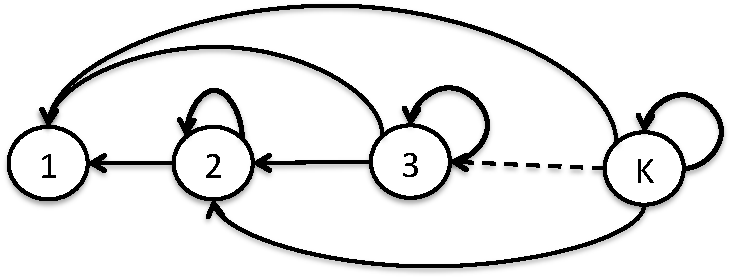
\includegraphics[scale=.4]{../Figures/SideInfoGraph.pdf}
	\caption{Side observation graph $G_S$. \todoc[inline]{Keeping the fig just in case.}}
	\label{fig:SideObservationGraph]}
\end{wrapfigure} 

%Let us now show how to reduce SAP under strong dominance to a specific 
%bandit with side-observations.
Let $\PSAP$ be the set of SAPs with action set $\A = [K]$.
The corresponding bandit problems will have the same action set,
while for action $k\in [K]$ the neighborhood set is $N(k) = [k]$.
Take any instance $(P,c)\in \PSAP$ and let $(Y,Y^1,\dots,Y^K) \sim P$ be the 
unobserved state of environment in round $s$.
We let the reward distribution for arm $k$ in the corresponding bandit problem
be a shifted Bernoulli distribution.
In particular, the cost of arm $k$ follows the distribution of 
$\one{Y^k\ne Y^1} + (c_1+\dots+c_k)$ (we use costs here to avoid flipping signs).
The costs for different arms are defined to be independent of each other.
Let $\Pside$ denote the set of resulting bandit problems and let $f:\PSAP \to \Pside$
be the map that transforms SAP instances to bandit instances by following the
transformation that was just described.
\todoc[inline]{
Ok, so if they are independent of each other, then the joint distributions will not be 
same as if they were not independent of each other.
Independence may lose information (e.g., may increase variance?).
If we define them not to be independent of each other, we will need to be careful
with the algorithms defined for bandits with side-observation: Do they use
(in their proof) independence of rewards underlying different arms?
I would think that they are not.
The downside of not defining independent rewards is that the specification of
bandits with side observations must allow this -- complicating things a bit in the background.
Another executive decision we should make is whether we like to see both costs and 
rewards.
}

Now let $\pi\in \Pi(\Pside)$ be a policy for $\Pside$.
Policy $\pi$ can also be used on any $(P,c)$ instance in $\PSAP$ in an obvious way:
In particular, given the history of actions and states $A_1,U_1,\dots,A_t,U_t$
in $\theta=(P,c)$ where $U_s = (Y_s,Y_s^1,\dots,Y_s^{K})$ such that 
the distribution of $U_s$ given that $A_s=a$ is $P$ marginalized to $\Y^{a}$,
the next action to be taken is 
$A_{t+1}\sim \pi(\cdot| A_1, V_1,\dots,A_t,V_t)$, where
$V_s = (\one{Y_s^1\ne Y_s^2}+c_1,\dots,\one{Y_s^1\ne Y_s^{A_s}}+c_1+\dots+c_{A_s})$. Let the resulting policy be denoted by $\pi'$.
The following can be checked by simple direct calculation:
\begin{proposition}
If $\theta \in \TWD$, then the regret of $\pi'$ on $f(\theta)\in \Pside$
is the same as the regret of $\pi$ on $\theta$. \todoc[inline]{We should probably add this
calculation?}
\end{proposition}
This implies that $\Regret_T^*(\TWD)\le \Regret_T^*(f(\TWD))$.

Now note that this reasoning can also be repeated in the other ``direction'': 
For this, first note that the map $f$ has a right inverse $g$ 
(thus, $f\circ g$ is the identity over $\Pside$)
and if $\pi'$ is a policy for $\PSAP$, 
then $\pi'$ can be ``used''  on any instance $\theta\in \Pside$
via the ``inverse'' of the above policy-transformation:
Given the sequence $(A_1,V_1,\dots,A_t,V_t)$ where 
$V_s= (B_s^1+c_1,\dots,B_ s^{K}+c_1+\dots+c_s)$ is the vector of costs for round $s$
with $B_s^k$ being a Bernoulli with parameter $\gamma_k$,
let $A_{t+1} \sim \pi'( \cdot| A_1,W_1,\dots,A_t,W_t)$ where
$W_s = (B_s^1,\dots,B_s^{A_s})$. Let the resulting policy be denoted by $\pi$.
Then the following holds:
\begin{proposition}
Let $\theta \in f(\TWD)$. Then the regret of policy $\pi$ on $\theta\in f(\TWD)$ is the same
as the regret of policy $\pi'$ on instance $f^{-1}(\theta)$.
\end{proposition}
Hence, $\Regret_T^*(f(\TWD))\le \Regret_T^*(\TWD)$.
In summary, we get the following result:
\begin{corollary}
$\Regret_T^*(\TWD) = \Regret_T^*(f(\TWD))$. 
\end{corollary}
\todoc[inline]{So this could in theory be used for upper and lower bounds.. 
However, $\Pside$ is really special (because of the fixed costs) -- hence it is unclear 
whether existing lower bounds, for example, would apply.
The next step could be to describe policies for bandits
with side observation starting from our paper with Yifan.
We have two types of policies.
One is asymptotically optimal, the other is minimax optimal.
Can we have a single policy in our special problem that would be simultanously 
optimal in both cases? What happens when only weak dominance
is satisfied?}

\if0
At the price of abusing notation 
we simplify the notation by dropping the indices from $f_{\A}, f_{\Y}$ and $f_{\Theta}$ (the identity of the appropriate map can be inferred from its argument).
Pick any policy $\pi_1\in \Pi_1$.s
First we define the policy corresponding to $\pi_1$.
Recall that a policy maps histories to distributions over actions.
Taking a history $(a_1,y_1,\dots,a_t,y_t)\in (\A_2\times \Y_2)^t$ ($t\ge 0$),
for $a_{t+1}\in \A_2$ we define the probability of taking $a_{t+1}$ by $\pi_2$, in notation,
 $\pi_2(a_{t+1}|a_1,y_1,\dots,a_t,y_t)$, as
 $\pi_2(a_{t+1}|a_1,y_1,\dots,a_t,y_t) = \pi_1(f(a_{t+1})|f(a_1),f(y_1),\dots,f(a_t),f(y_t))$.
Pick any instance $\theta_2 = (p',r')\in \Theta_2$ and let $(p,r) = \theta_1  = f( \theta_2)$.
The probability distribution over histories $\Y_1 \times \A_1$ generated by $\pi_1$ and $\theta_1$
\fi





\section{Experiments}
\label{sec:Experiments}
%\vspace{-10pt}
%
%In this section we evaluate performance of Algorithms \ref{alg:asym} and \ref{alg:UCB} on synthetic and real datasets. For synthetic example, we consider data transmission over a binary symmetric channel, and for real world examples, we use diabetes (PIMA indiana) and heart disease (Clevland) from UCI dataset. In both datasets attributes/features are associated with costs, where features related to physical observations are cheap and that obtained from medical tests are costly. The experiments are setup as follows:
%
%{\bf Synthetic:} we consider data transmission over three binary symmetric channels (BSCs). Channel $i=1,2,3$ flips input bit with probability $p_i$ where $p_1\geq p_2\geq p_3$. Transmission over channel $1$ is free and that over channel $2$ and $3$ costs price of $ c_2$ and $c_3\in (0,1] $ units per bit, respectively. Input bits are generated with probability $0.7$ and we set $p_1=.4, p_2=.1$ and $p_3=.05$.
%
%{\bf Datatsets:} we obtain a \ses setup from the datasets as follows: Three svm classifiers (linear, $C=.01$) are trained for each dataset, first one using only cheap features, second one  using cheap features plus few additional features and the third one using all features. These classifiers form sensors of a three stage SAP where classifier trained with cheap features is the first stage and that trained with all the features forms the last stage. Cost of each stage is the sum of cost of features used to train that stage multiplied by a scaling factor $\lambda$ (trade-off parameter between prediction accuracy and costs). Specific details for each dataset is given below.  
%
%{\bf PIMA indians diabetes} dataset consists of $768$ instances and has $8$ attributes. The labels identify if the instances are diabetic or not. First sensor of SAP is trained with $4$ cheap attributes and costs \$$4$ (times-pregency, pedigree, diastolic-pb, triceps ). Second sensor is trained from $7$ attributes that includes age, mass-index and insulin in addition to the attributed used for the first sensor and cost total of \$$29$, and the last sesnor is trained with all $8$ attributes that cost \$$46$. We set $C_1= 4\lambda, C_2= 29\lambda$ and $C_3= 46\lambda$.
%% $6$ of the attributes obtained from physical observations are cheap, and $2$ attributes (glucose and insulin) require expensive tests. 
%
%{\bf Heart disease} dataset consists of $297$ instance (without missing values) and has $13$ attributes. $5$ class labels $(0,1,2,3,4)$ are mapped to binary values by taking value $0$ as `absence' of disease and values $(1,2,3,4)$ as `presence' of disease. First senor of SAP is trained with first $7$ attributes which cost  \$$32$ in total, second sensor is trained with first $11$ attributes that cost \$$1$ each and the third sensor is trained with all the attributes  cost total of \$$568$. We set $C_1= 32\lambda, C_2= 397\lambda$ and $C_3= 601\lambda$.
%=======
%\begin{figure*}[!bt]
%	\begin{minipage}{4cm}
%		\centering
%		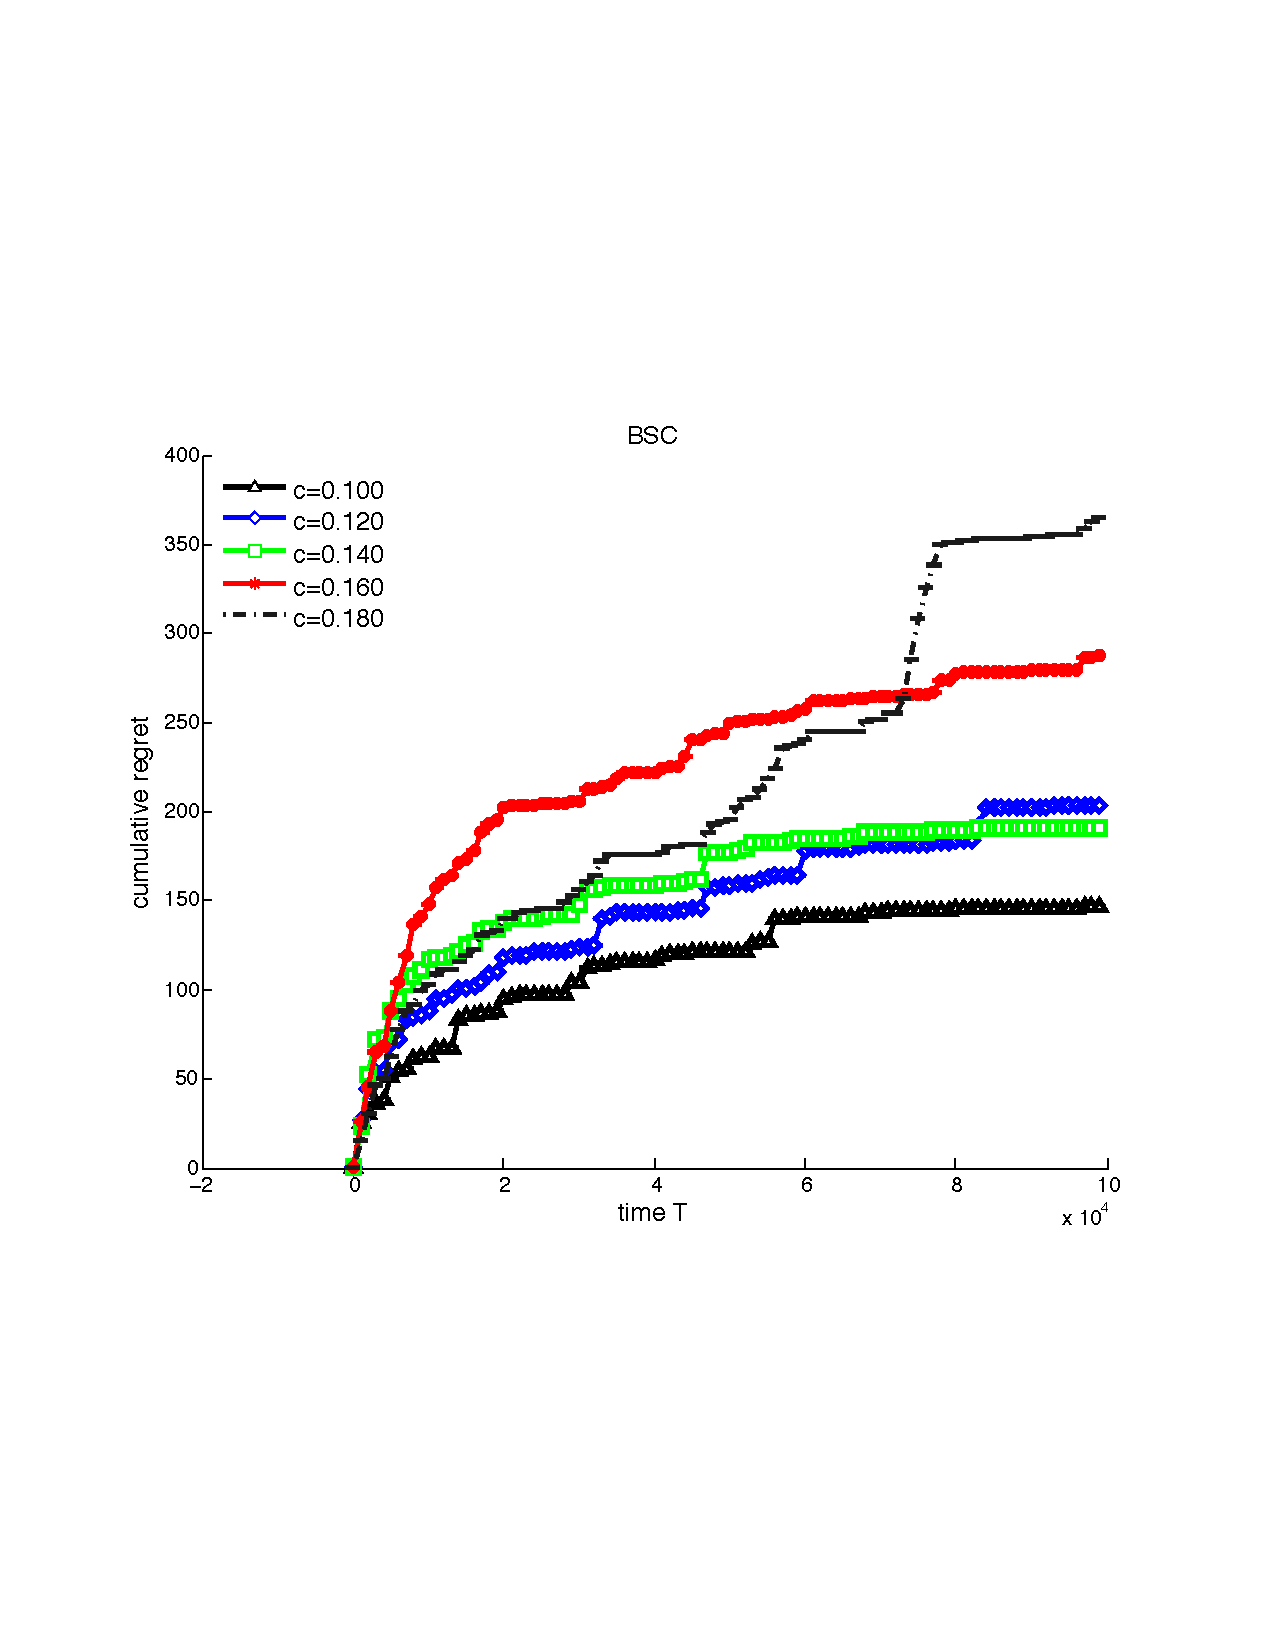
\includegraphics[scale=0.2]{../Simulations/Figures/BSC_SD}
%		\label{fig:BSC1}
%		\caption{BSC wtih SD}
%	\end{minipage}
%	\begin{minipage}{4cm}
%		\centering
%		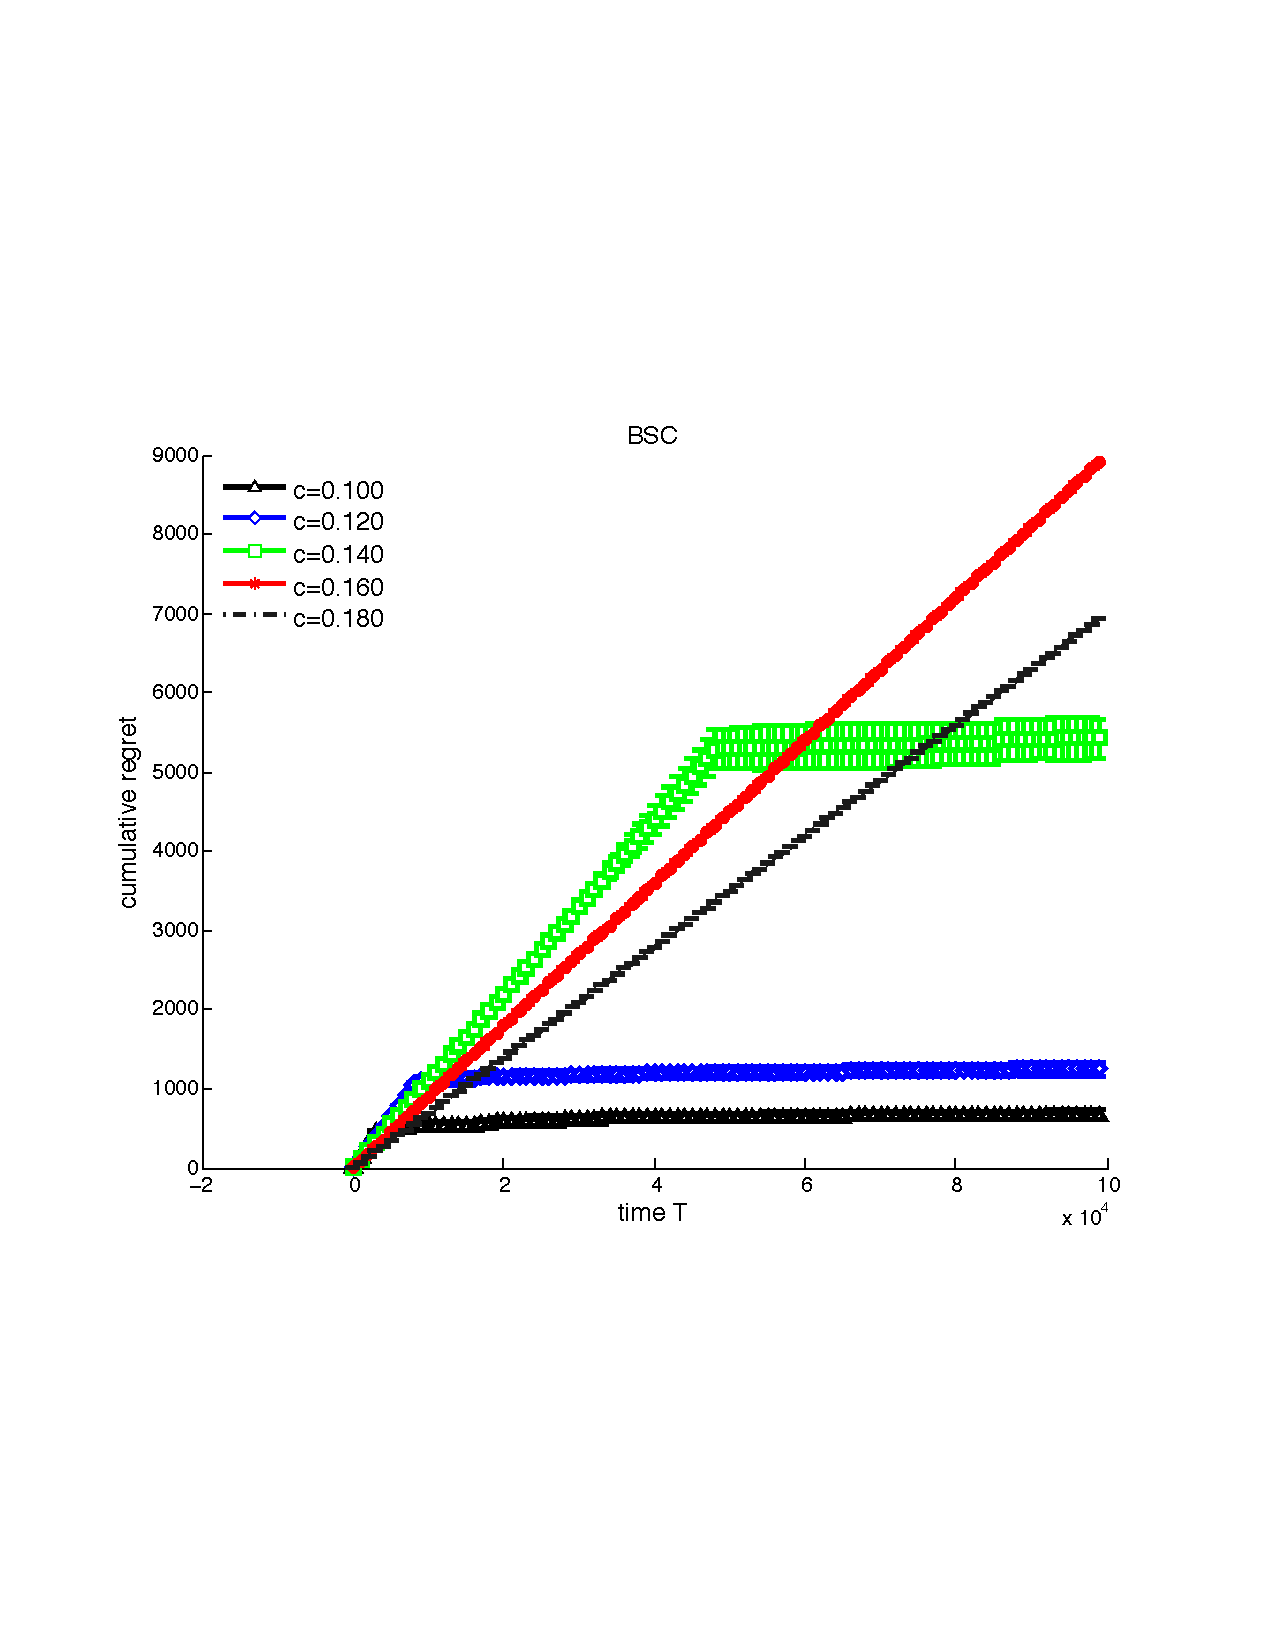
\includegraphics[scale=0.2]{../Simulations/Figures/BSC_WD}
%		\label{fig:BSC2}
%		\caption{BSC dataset}
%	\end{minipage}
%	\begin{minipage}{4cm}
%		\centering
%		\includegraphics[scale=0.2]{../Simulations/Figures/Heart}
%		\label{fig:Heart}
%		\caption{BSC dataset}
%	\end{minipage}
%	\begin{minipage}{4cm}
%		\centering
%		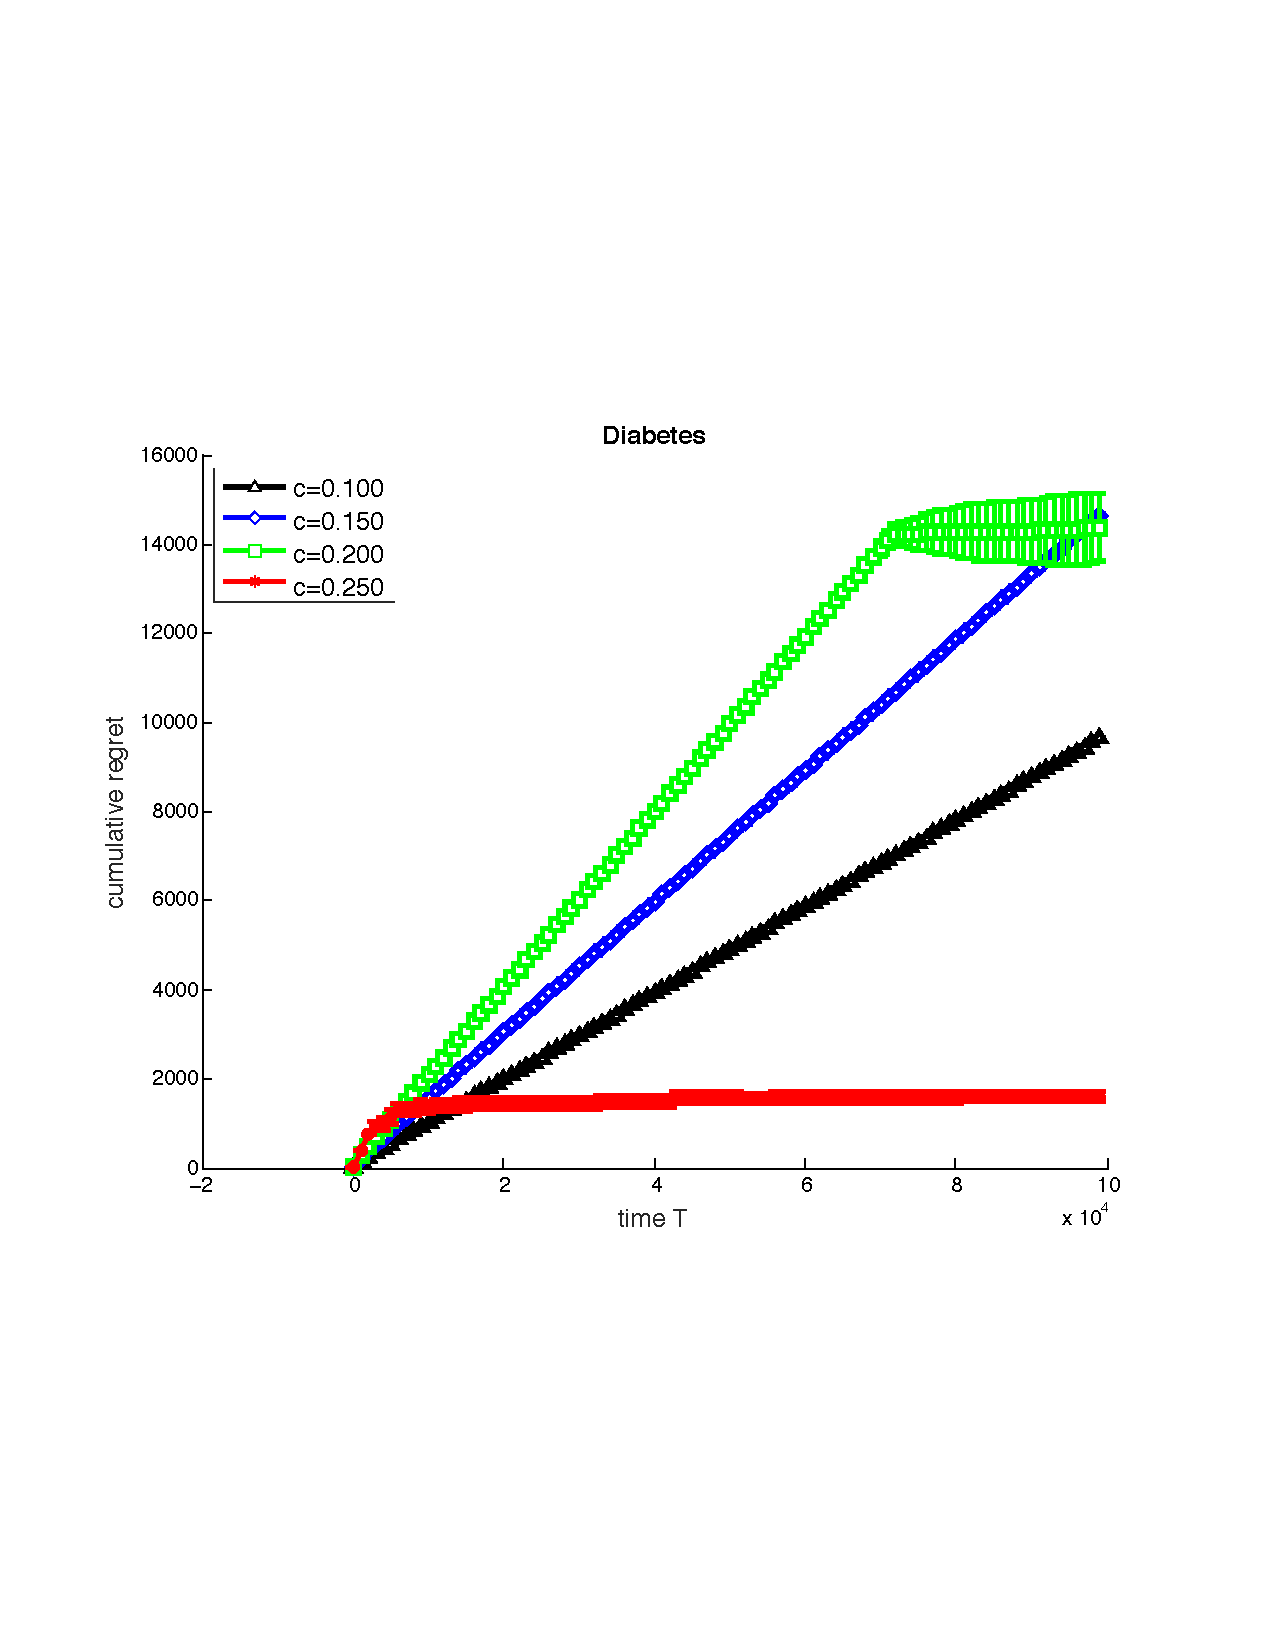
\includegraphics[scale=0.2]{../Simulations/Figures/Diabetes_WD}
%		\label{fig:Heart}
%		\caption{Heart dataset}
%	\end{minipage}
%	\vspace{.2cm}

%\noindent
%In Fig. \ref{fig:BSC1}, BSC data is generated that satisfies SD property and Algorithm \ref{alg:asym} is applied. In  Fig. \ref{fig:BSC2}, Algorithm \ref{alg:UCB} is applied on BSC data. In Fig. \ref{fig:BSC3}, true labels are used and standard UCB algorithm is applied on BSC dataset. In Fig. \ref{fig:Heart}, we applied Algorithm \ref{algo:UCB} on the heart dataset. 
%\end{figure*}
%
In this section we evaluate performance of Algorithms \ref{alg:asym} and \ref{alg:UCB} on synthetic and real datasets (PIMA-Diabetes) and Heart Disease (Cleveland). Both of these datasets have accompanying costs for individual features.%. For synthetic example, we consider a binary symmetric channel, and for real world examples, we use diabetes (PIMA indiana) and heart disease (Clevland) from UCI dataset. In both datasets attributes/features are associated with costs, where features related to physical observations are cheap and that obtained from medical tests are costly. The experiments are setup as follows:

{\bf Synthetic:} We generate data as follows. The input, $Y_t$, is generated IID Ber($0.7$). Outputs for channels 1, 2, 3 have an overall error statistic, $\gamma_1 = 0.4,\,\gamma_2=0.1,\,\gamma_3=0.05$ respectively. To ensure SD we enforce Defn.~\ref{eqn:DominanceCondition} during the generation process. To relax SD requirement we introduce errors upto 10\% during data generation for sensor outputs 2 and 3 when sensor 1 predicts correctly.% (while still maintaint the overall error).  

%Channel $i=1,2,3$ flips input bit with probability $p_i$ where $p_1\geq p_2\geq p_3$. Transmission over channel $1$ is free and that over channel $2$ and $3$ costs price of $ c_2$ and $c_3\in (0,1] $ units per bit, respectively. Input bits are generated with probability $0.7$ and we set $p_1=.3, p_2=.1$ and $p_3=.05$.

{\bf Real Datasets:} %we obtain a \ses setup from the datasets as follows: 
We split the features into three ``sensors'' based on their costs. For PIMA-Diabetes dataset (size=$768$) the first sensor is associated with patient history/profile with cost (\$6), the 2nd sensor in addition utilizes  insulin test (cost \$ 22) and the 3rd sensor uses all attributes (cost \$46). For the Heart dataset (size=$297$) we use the first $7$ attributes that includes cholestrol readings, blood-sugar, and rest-ECG (Cost \$27), the 2nd sensor utilizes in addition thalach, exang, oldpeak attributes that cost $\$300$  and the 3rd sensor utilizes more extensive tests at a total cost of \$601. 


We train three linear SVM classifiers with 5-fold cross-validation and have verified that our results match known state-of-art. Note that Table~\ref{tab:ErrorTable1} shows that the resulting classifiers/tests on these datasets approximately satisfies SD condition and thus our setup should apply to these datasets. 
%
%
%The (linear, $C=.01$) are trained for each dataset, first one using only cheap features, second one  using cheap features plus few additional features and the third one using all features. These classifiers form sensors of a three stage SAP where classifier trained with cheap features is the first stage and that trained with all features forms the last stage. Cost of each stage is the sum of cost of features used to train that stage multiplied by a scaling factor $\lambda$ (trade-off parameter for accuracy and costs). Specific details for each dataset is given below.  
%
%{\bf PIMA indians diabetes} dataset consists of $768$ instances and has $8$ attributes. The labels identify if the instances are diabetic or not. $6$ of the attributes (age, sex, triceps, etc.) obtained from physical observations are cheap, and $2$ attributes (glucose and insulin) require expensive tests. First sensor of SAP is trained with $4$ cheap attributes and costs \$$4$. Second sensor is trained from $6$ attributes that cost \$$6$, and the last sesnor is trained with all $8$ attributes that cost \$$6$. We set $C_1= 4\lambda, C_2= 6\lambda$ and $C_3= 30\lambda$.
%
%{\bf Heart disease} dataset consists of $297$ instance (without missing values) and has $13$ attributes. $5$ class labels $(0,1,2,3,4)$ are mapped to binary values by taking value $0$ as `absence' of disease and values $(1,2,3,4)$ as `presence' of disease. First senor of SAP is trained with $4$ attributes which cost  \$$1$ each and second sensor is trained with $8$ attributes that cost \$$1$ each. Total cost of all attributes is \$$568$. We set $C_1= 7\lambda, C_2= 8\lambda$ and $C_3= 568\lambda$.
%
%Various error probabilities for synthetic and datasets are listed in Table (\ref{tab:ErrorTable}).  
%	\begin{figure}[!h]
%		\small
%		\begin{tabular}[c]{c|c|c|c|c|c|c } 
%			\label{tab:ErrorTable}
%			%	\caption{cap:Error statistics}
%			dataset & $\gamma_1$ & $\gamma_2$ & $\gamma_3$ &$\delta_{12}$ & $\delta_{13}$ & $\delta_{23}$ \\ \hline 
%			BSC & .3 & .1 & .05 & .07 & .035 & .045\\  \hline
%			diabetic & $0.345 $ & $ 0.324$ & 0.246 & $ 0.116 $ & 0.089 &0.058\\  \hline
%			heart & $0.292$ & $0.27$ & 0.146 & $0.124$ & 0.067 & 0.079\\  \hline
%		\end{tabular}
%		\caption{Error statistics for real and synthetic datasets. $\delta_{ij}\defeq\P\{Y_j\neq Y \mid Y_i = Y\}$.}
%\label{tab:error_stats}
%\vspace{-.5cm}
%	\end{figure}
The size of these datasets is relatively small and limits our ability to experiment. To run the online algorithm we therefore generate an instance randomly from the dataset (with replacement) in each round. We repeat the experiments $20$ times and averages are shown with $95\%$ confidence bounds.

\begin{center}
\begin{figure*}[!bt]
%\vspace{-10pt}	
\begin{minipage}{8cm}
		\centering
		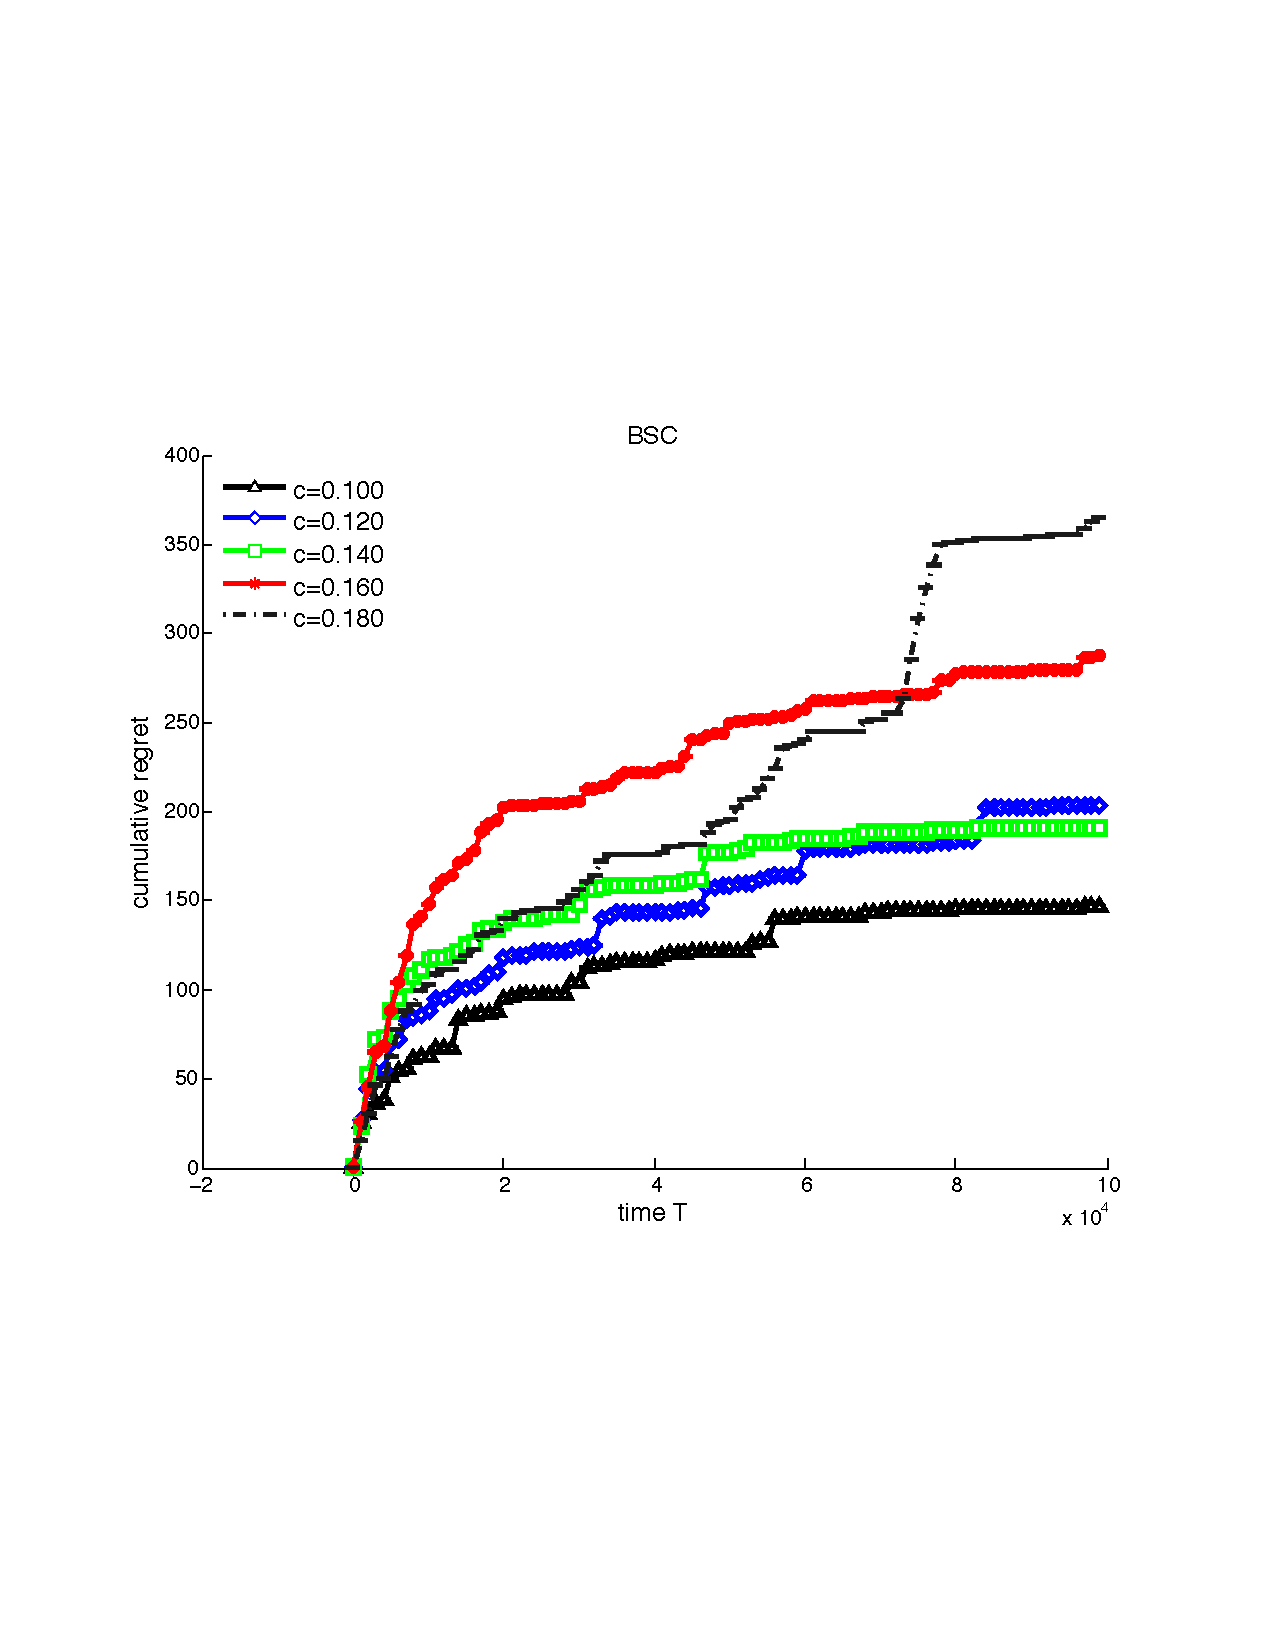
\includegraphics[scale=0.4]{../Simulations/Figures/BSC_SD}
				\vspace{-.3cm}
		\caption{\footnotesize Regret under SD property}
\label{fig:BSC_SD}
	\end{minipage}
	\begin{minipage}{8cm}
		\centering
		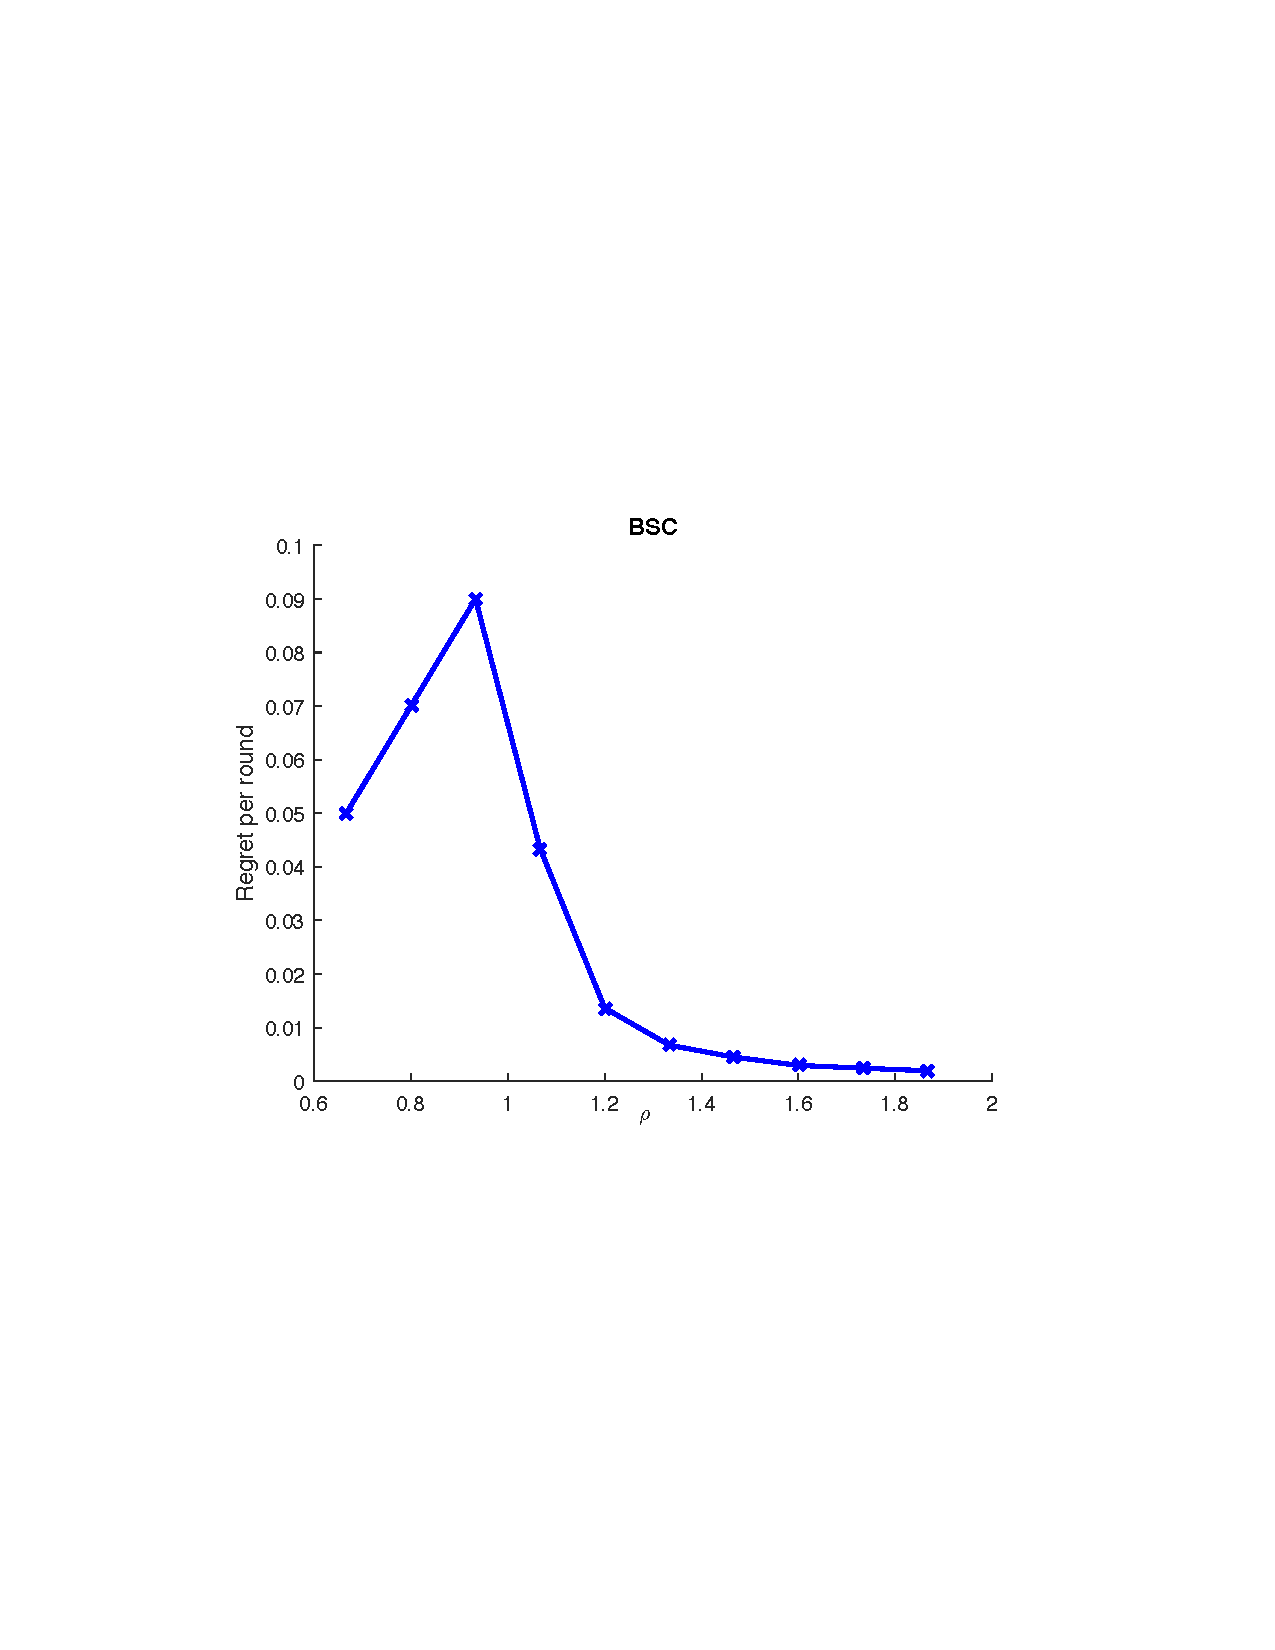
\includegraphics[scale=0.4]{../Simulations/Figures/BSC_WD1}
				\vspace{-.3cm}
		\caption{\footnotesize Regret under varying levels WD condition}
\label{fig:BSC_WD}
	\end{minipage}
%	\begin{minipage}{4cm}
%		\centering
%		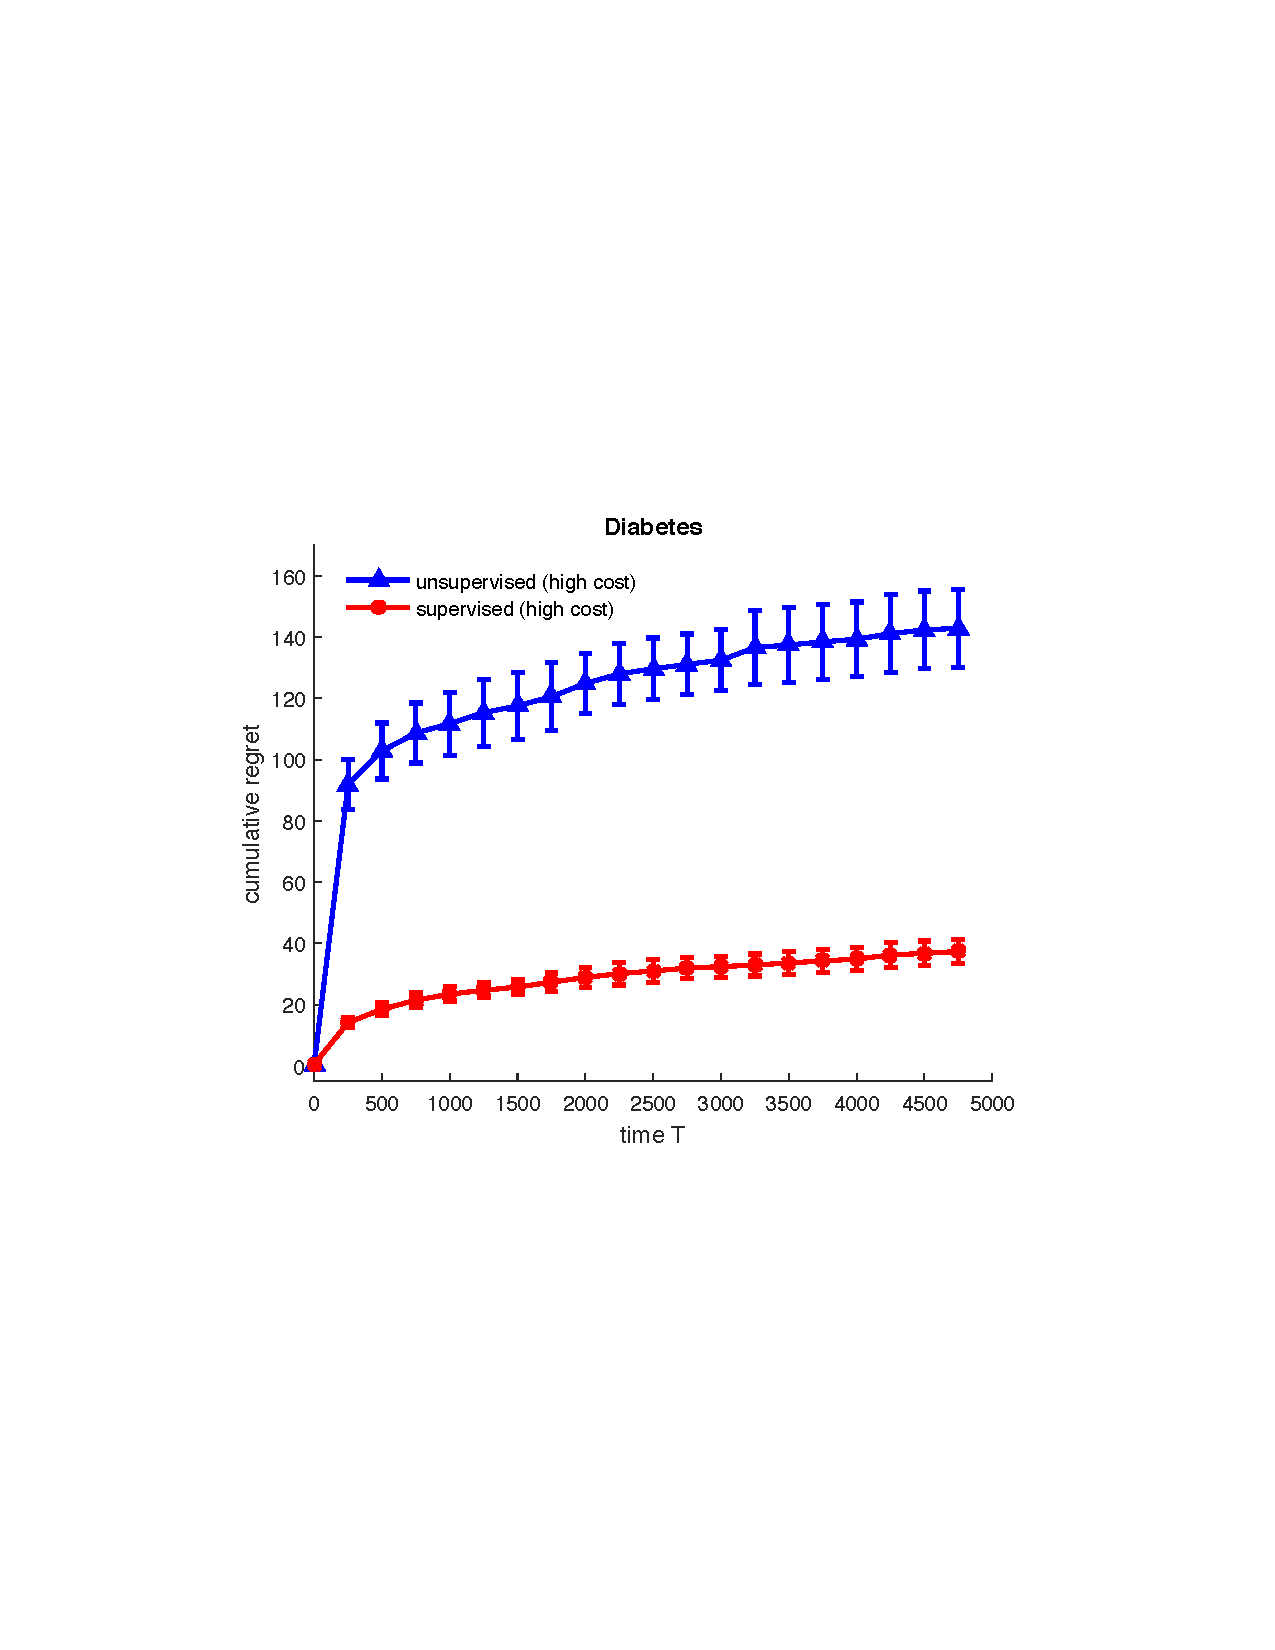
\includegraphics[scale=0.3]{../Simulations/Figures/Diabetes_WD1}
%		\vspace{-.3cm}
%		\caption{\footnotesize {\bf PIMA Diabetes}}
%		\label{fig:Diabetes}
%	\end{minipage}
%	\begin{minipage}{4cm}
%		\centering
%	%	\vspace{.2cm}
%		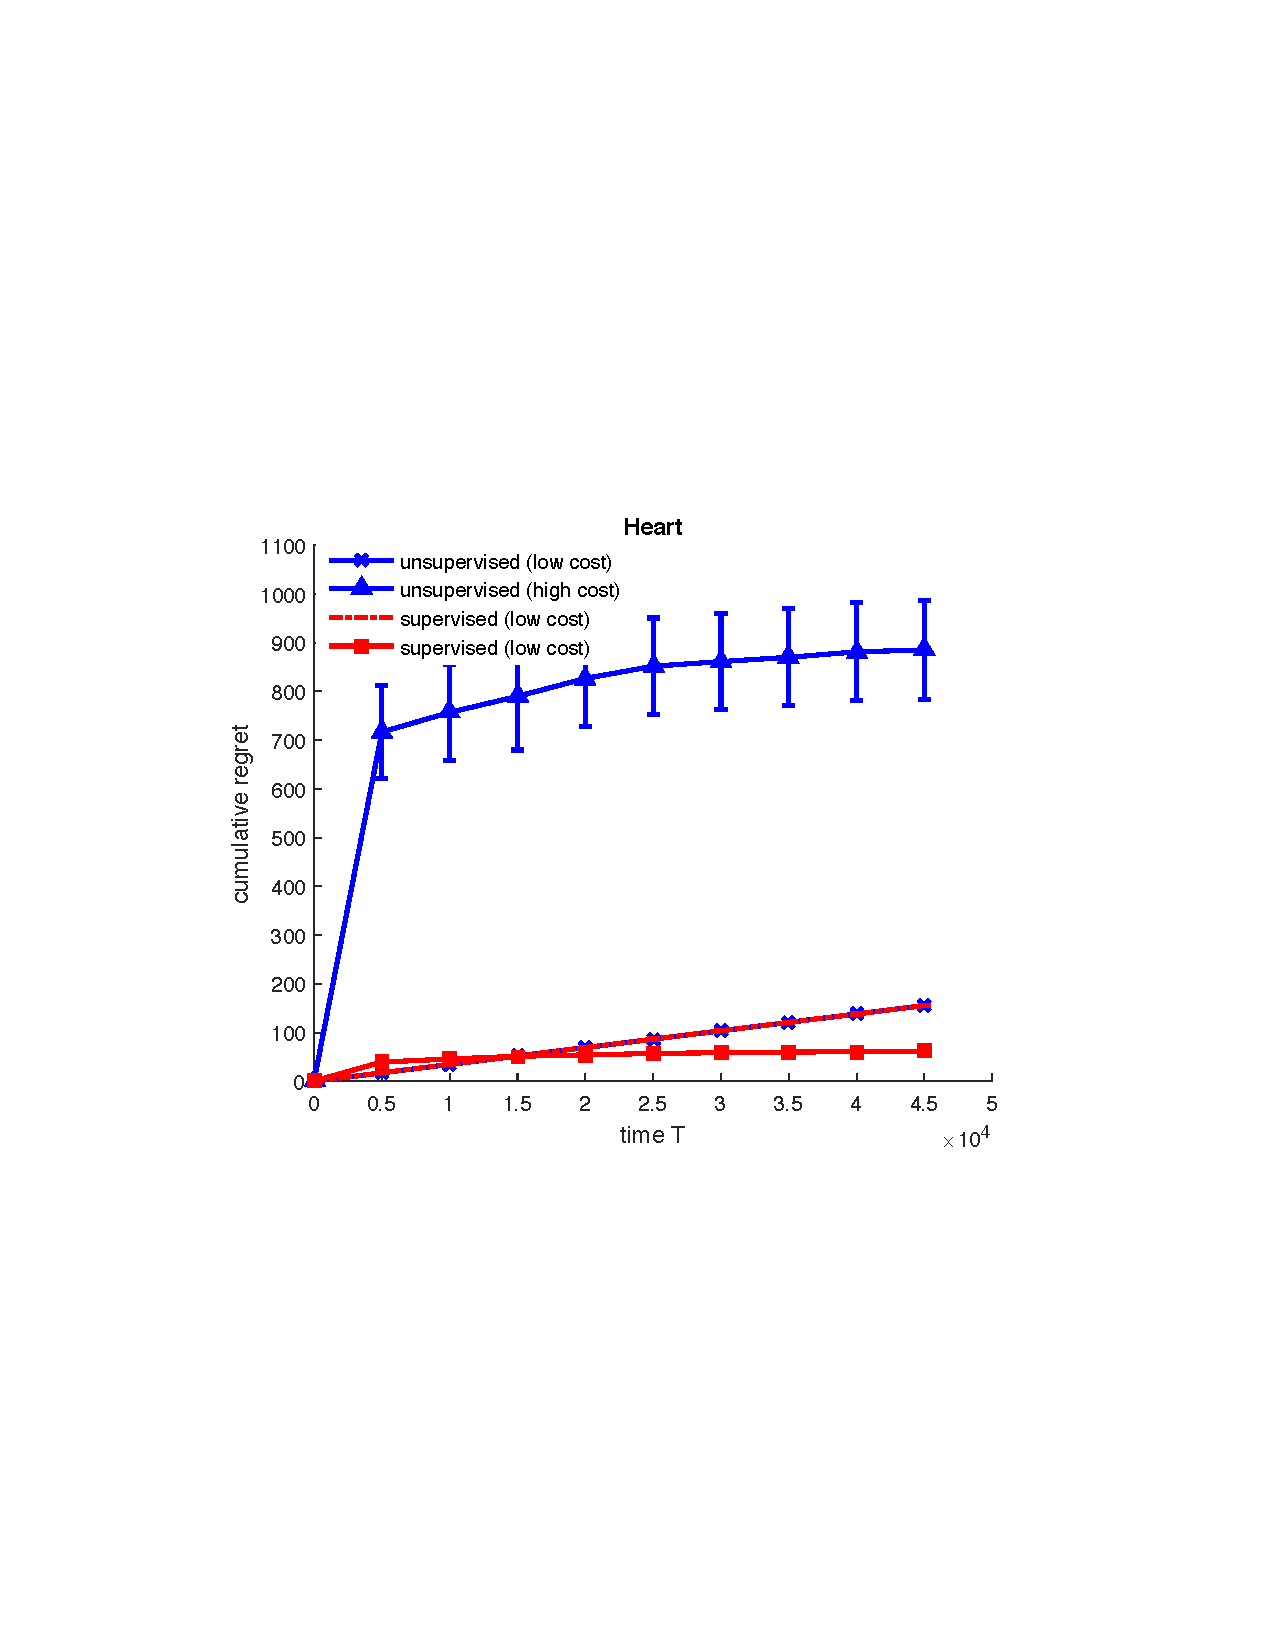
\includegraphics[scale=0.3]{../Simulations/Figures/Heart_WD1}
%%		\vspace{-.5cm}
%		\caption{\footnotesize {\bf Heart Disease}}
%	\label{fig:Heart}
%%\vspace{-.3cm}
%	\end{minipage}
	%\vspace{.3cm}
%
\vspace{5pt}

\noindent
{\footnotesize Fig. \ref{fig:BSC_SD} depicts regret of USS (Alg.~1) on synthetic data. Under SD it is always sublinear regardless of costs/probability. Fig. \ref{fig:BSC_WD} demonstrates phase-transition effect for USS (Alg.~2). Alg.~1 is not plotted here because it fails in this case. As $\rho \rightarrow 1$ (from the right) regret-per-round drastically increases thus validating our theory that WD is a maximal learnable set. 
%, Algorithm \ref{alg:UCB} is applied on BSC data. In Fig. \ref{fig:Diabetes} Algorithm \ref{alg:UCB} and the standard UCB algorithm that uses ground truth are applied on the Diabetes dataset. In Fig. \ref{fig:Heart}, same experiment is repeated on the heart dataset.
}
%\vspace{-15pt}
\end{figure*}
\end{center}

\begin{center}
	\begin{figure*}
		\begin{minipage}{8cm}
			\centering
			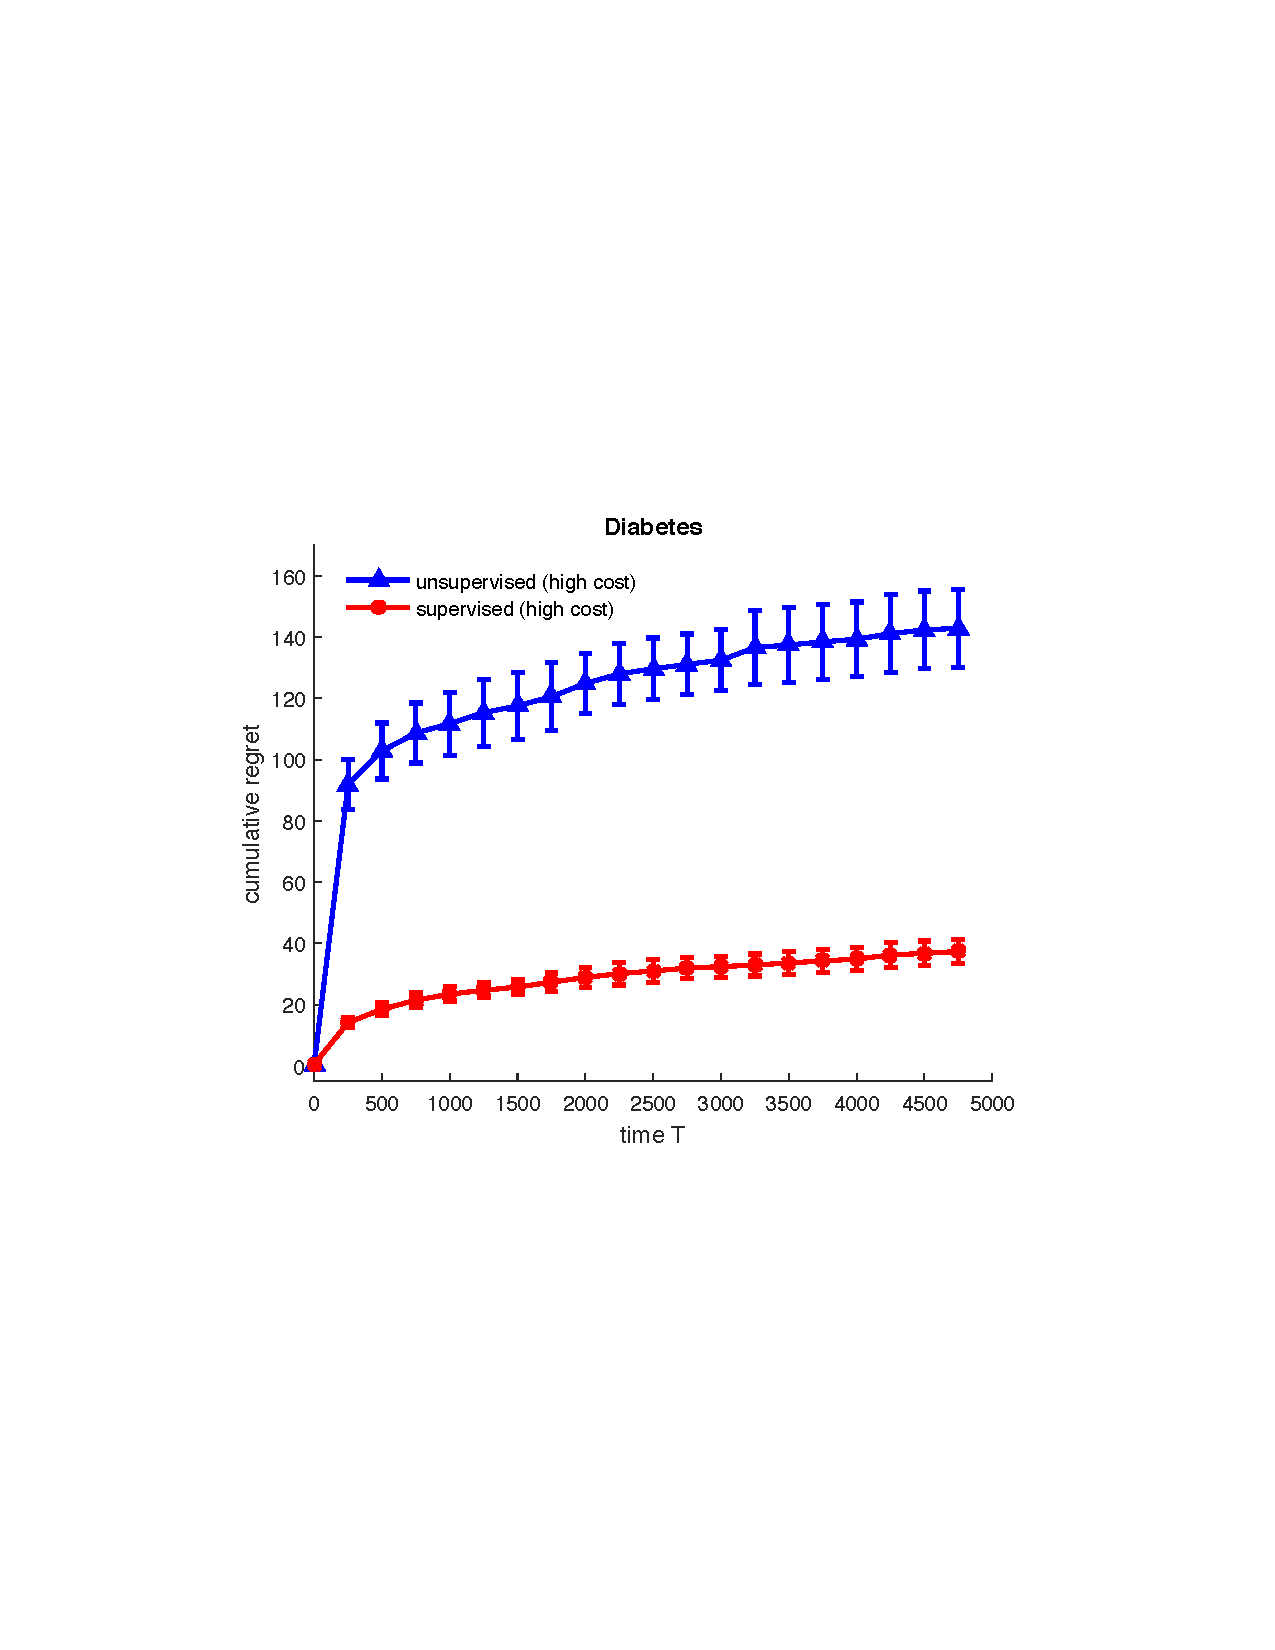
\includegraphics[scale=0.4]{../Simulations/Figures/Diabetes_WD1}
			\vspace{-.3cm}
			\caption{\footnotesize Regret Curves on PIMA Diabetes}
			\label{fig:Diabetes}
		\end{minipage}
		\begin{minipage}{8cm}
			\centering
			%	\vspace{.2cm}
			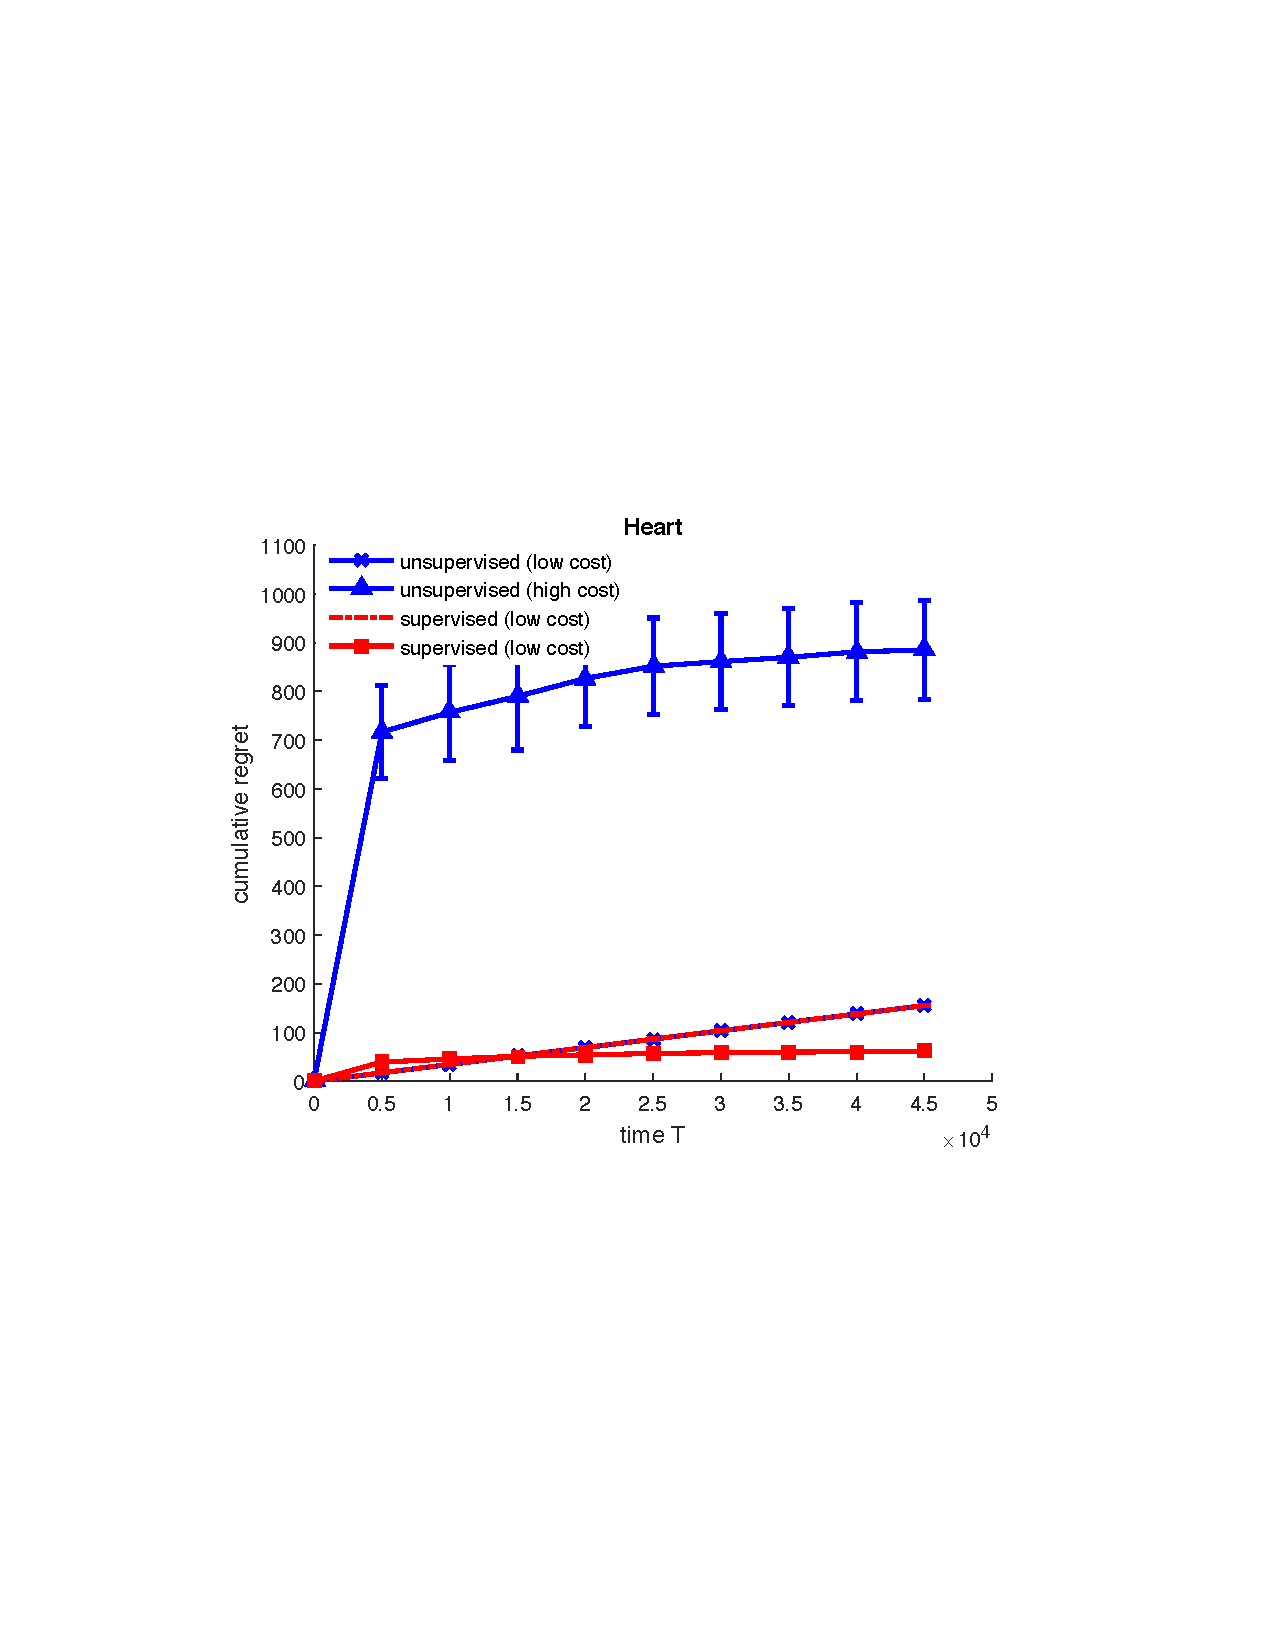
\includegraphics[scale=0.4]{../Simulations/Figures/Heart_WD1}
			\vspace{-.3cm}
			\caption{Regret Curves on Heart Disease}
			\label{fig:Heart}
			%\vspace{-.3cm}
		\end{minipage}
		\vspace{5pt}
		
		\noindent
		{\footnotesize Fig. \ref{fig:Diabetes} and Fig. \ref{fig:Heart} depict performance for real-datasets and presents comparisons against supervised (bandit with ground-truth feedback) scenario. Typically (but not in the worst-case (see Thm~5)), under WD, the unsupervised learning rate is within a constant factor of supervised setting.
			%, Algorithm \ref{alg:UCB} is applied on BSC data. In Fig. \ref{fig:Diabetes} Algorithm \ref{alg:UCB} and the standard UCB algorithm that uses ground truth are applied on the Diabetes dataset. In Fig. \ref{fig:Heart}, same experiment is repeated on the heart dataset.
		}
	\end{figure*}
\end{center}
\vspace{-1.5cm}
\noindent
{\bf Testing Learnability:}
We experiment with different USS algorithms on the synthetic dataset. Our purpose is twofold: (a) verify sublinear regret reduction scheme (Alg~1) under SD (b) verify that WD condition is a maximal learnable set. 
Fig.~\ref{fig:BSC_SD} depicts the results of Alg.~\ref{alg:asym} when SD condition is satisfied and shows that we obtain sublinear regret regardless of costs/probabilities. To test WD requirement we parameterize the problem by varying costs. Without loss of generality we fix the cost of sensor 1 to be zero and the total cost of the entire system to be $C_{\mbox{tot}}$. We then vary cost of sensors 2 and 3. %To plot the effect of WD we note from Eq.~\ref{eqn:WD} that for an optimal sensor $i$, $\rho \geq 1$. 
%we must have that if optimal sensor $i <K$ then the ratio,
%$$
%\rho = \min_{i < j} \frac{(c_j - c_i)}{\Pr\{Y^j \neq Y^i\}} \geq 1.
%$$
%This corresponds to the condition that the worst-case marginal-cost to marginal absolute error is bounded by 1.
We test the hypothesis that WD is a maximal learnable set. We enforce Sensor 2 as the optimal sensor and vary the costs so that we continuously pass from the situation where WD holds ($\rho \geq 1$) to the case where WD does not hold ($\rho < 1$). %The optimal arm is correctly identified for all costs. 
Fig.~\ref{fig:BSC_WD} depicts regret-per-round for Alg.~\ref{alg:UCB} and as we can verify there is indeed a transition at $\rho = 1$ . %While for SD condition Alg.~\ref{alg:asym} is superior there is an inherent lack of robustness when SD fails to be satisfied. Consequently,  Alg.~\ref{alg:UCB} is somewhat more robust to relaxation of SD assumption.

\noindent
{\bf Unsupervised vs. Supervised Learning:}
The real datasets provide an opportunity to understand how different types of information can impact performance. We compare USS algorithm (Alg.~2) against a corresponding bandit algorithm where the learner receives feedback. In particular, for each action in each round, in the bandit setting, the learner knows whether or not the corresponding sensor output is correct. We implement the supervised bandit setting by replacing Step 5 in Alg.~2 with estimated marginal error rates. 

We scale costs by means of a tuning parameter (since the costs of features are all greater than one) and consider minimizing a combined objective ($\lambda$ Cost + Error) as stated in Sec.~2. High (low)-values for $\lambda$ correspond to low (high)-budget constraint. If we set a fixed budget of (\$ 50), this corresponds to high-budget (small $\lambda$) and low budget (large $\lambda$) for PIMA Diabetes (3rd test optimal) and Heart Disease (1st test optimal) respectively. Figs~\ref{fig:Diabetes} and \ref{fig:Heart} depicts performance for typical scenarios. We notice that for both high as well as low cost scenarios, while supervised does have lower regret, the USS cummulative regret is also sublinear and within a constant fraction of the supervised case. This is qualititively interesting because these plots demonstrate that (although under WD we do not have uniform learnability), in typical cases, we learn as well as the supervised setting. %as in the supervised bandit setting. In general we emphasize that in many medical and security systems it is often difficult to obtain ground-truth annotatations for examples.



%Our objective is to choose a sensor that minimizes 
%
%We  (Alg.~\ref{alg:UCB}) (unsuprvised) against UCB bandit algorithm that observes reward for each action (supervised). Note that for USS we apply Alg.~\ref{alg:UCB} because the real datasets does not satisfy SD condition and our experience on synthetic data (see Fig.~\ref{fig:BSC_WD}). Our implementation for UCB algorithm is based on modification of Alg.~\ref{alg:UCB}) that keeps track of error rates of each arm by  directly utilizing ground truth $Y$ rather than pairwise-disagreements (Step 5 in Alg.~\ref{alg:UCB}). We benchmark the performance with respect to a budget constrained problem, where the objective is to pick a sensor that minimizes error with respect to a budget constraint. We consider both high and low available budget situations. For Heart and Diabetes datasets a low budget is about (\$ 10). We note from the error probabilities in Table~\ref{tab:error_stats} that the optimal sensor in such a situation is Sensor 1. On the other hand for a budget of about (\$ 50) the optimal sensor for Diabetes dataset is Sensor 3, while for the Heart dataset it is Sensor 2. To map this to our setting we consider an equivalent error-cost tradeoff objective ($\lambda$ Cost + Error) with an appropriate scaling parameter $\lambda$ so that it leads to the same sensor choice based on Eq.~\ref{eqn:interp_opt} as in the constrained one. We then compare supervised and unsupervised scenarios in Figs~\ref{fig:Diabetes} and \ref{fig:Heart} for real datasets. We notice that for both high as well as low cost scenarios, while supervised does have lower regret, the cummulative regret is also sublinear and within a constant fraction of the regret for unsupervised case. This is qualititively interesting because these plots demonstrate that (although under WD we do not have uniform learnability) in typical cases we learn in unsupervised setting as in the supervised bandit setting. In general we emphasize that in many medical and security systems it is often difficult to obtain ground-truth annotatations for examples.


%Fo the synthetic experiments we set $c_1=0$ and $c_2+c_3=0.4$ while varying $c_2$ from $0.1$ to $0.29$. The optimal action in this setup is $2$. In Figure \ref{fig:BSC_SD} we applied Algorithm \ref{alg:asym} on BSC data that satisfies SD property. As seen, the algorithm learns the optimal arm for all values of $c_2$. In Fig. ~\ref{fig:BSC_WD} 
%we applied Alg. ~\ref{alg:UCB} on BSC data, where $x$-axis in the figure is the ratio
%\[R= \frac{0.4 - c_2}{\Pr\{Y^2 \neq Y^3\}}\]
%and $y$-axis is the regret per round. As shown, regret per round is small when $R>1$, whereas it is high for $R<1$. This observation follows by applying definition of (\ref{dfn:WDP})- when $R>1$, the setup satisfies the WD property and the algorithm identifies the optimal action, whereas when $R<1$ the setup violates the WD property and the algorithm cannot identify the optimal arm resulting in high regret per round. This validates the learnability under the WD property. 

%In figure \ref{fig:Diabetes}, we apply Algorithm $2$ and the standard UCB algorithm on the Diabetes dataset. In applying the standard using algorithm, we use the true label in each round to get the loss for the action played. The regret plots corresponding to the Algorithm $2$ are labeled as unsupervised and that corresponding to standard UCB as supervised in the figure. We consider two values for trade-off factor, $\lambda=0.001$ and $\lambda=0.015$. In the first case, accuracy is given higher weight and action $3$ is optimal, in the second cost factor becomes dominant and action $1$ is optimal. When action $3$ is optimal, the performance of both the supervised and unsupervised methods are almost identical. When action $1$ is optimal. As expected, the performance of unsupervised method is better than the supervised method, but unsupervised method learns the optimal arms almost after the same number of rounds as the supervised method though it incurs high regret in the initial rounds.


%In figure \ref{fig:Heart} we again apply Algorithm $2$ on the standard UCB algorithm on the heart dataset. We set $\lambda=0.05$ for which action $1$ is optimal. The two corresponding plots are labeled as unsupervised and supervised in the figure. We also plot the regret obtained when noisy labels are input to the 
%the standard UCB algorithm instead of the true labels. This plot is labeled as supervised (noisy) in the figure which is obtained when each label is flipped by probability $0.2$. As seen, the regret performance of the supervised method deteriorates as label gets noisier. 


%and the average is shown in figures (\ref{fig:BSC1}-\ref{fig:Heart}) with $95\%$ confidence bounds. The left Figure in\ref{fig: BSC1} we applied Algorithm \ref{alg:asym} on BSC data that satisfies SD property. As see, the algorithm learns the optimal arm. In Figure \ref{fig:BSC2} 
%we applied Algorithm \ref{alg:UCB} on BSC data where we fixed $c_1=0$ and $c_2+c_3=0.3$ while varying $c_2$ between $0.1$ $0.18$. For all the cost values, arm $2$ is optimal. When $c_2 \in \{0.1, 0.12,  0.14\}$ the weak dominance property is satisfied and the algorithm learns the optimal arm. For values $c_2 \in \{0.16, 0.18\}$ weak dominance property is violated we get linear regret as shown in the plots. In figure  \ref{fig:BSC3} we use the standard UCB algorithm that has access to the true labels and knows the if a sensor made error. As seen this setting learns much faster than than compared to unsupervised algorithm shown in figure \ref{fig:BSC1} and \ref{fig:BSC2}. In figure we apply Algorithm \ref{algo:UCB} on diabetes dataset varying the trade-off factor $\lambda$. In the regions where WD property holds, the algorithm identifies the optimal arm.

\newpage
\bibliographystyle{biblio}
%\bibliographystyle{IEEEtran}
\bibliography{bandits1}


\newpage
\section{Appendix}

%\section{Proof of Theorem \ref{thm:K-SAPRegret}}
Consider a $K$-armed stochastic bandit problem where reward distribution $\nu_i$ has mean  $\gamma_1-\gamma_i- \sum_{j< i}c_j$ for all $i >1$ and arm $1$ gives a fixed reward of value $0$. The arms have side-observation structure defined by graph $G_S$.  
Given an arbitrary policy $\pi=(\pi_1, \pi_2, \cdots \pi_t )$ for the SAP, we obtain a policy for the bandit problem with side observation graph $G_S$ from $\pi$ as follows: Let $H_{t-1}$ denote the history, consisting of all arms played and the corresponding rewards, available to policy $\pi_{t-1}$ till time $t-2$. In round $t-1$, let $a_{t-1}$ denote the arm selected by the bandit policy,  $r_{t-1}$ the corresponding reward and $o_{t-1}$ the side-observation defined by graph $G_S$. Then, the next action $a_t$ is obtained as follows:
\begin{equation}
\label{eqn:SAPtoKBandit}
a_t=
\begin{cases}
\pi_t(H_{t-1}\cup \{1, \emptyset
\}) \mbox{ if } a_{t-1}= \mbox{arm 1}	\\
\pi_t(H_{t-1} \cup \{i, r_{t-1}\cup o_{t-1}\}) \mbox{ if } a_{t-1}= \mbox{arm i}
\end{cases}
\end{equation}
\noindent
Conversely, let $\pi^\prime=\{\pi^\prime_1, \pi^\prime_2,\cdots\}$ denote an arbitrary policy for the $K$-armed bandit problem with side-observation graph. we obtain a policy the SAP as follows: Let $H^\prime_{t-1}$ denote the history, consisting of all actions played and feedback, available to policy $\pi^\prime_{t-1}$ till time $t-2$. Let $a^\prime_{t-1}$ denote the action selected by the SAP policy in round $t-1$ and observed feedback $F_t$. Then, the next action $a^\prime_t$ is obtained as follows:
\begin{equation}
\label{eqn:KBanditToSAP}
a^\prime_t=
\begin{cases}
\pi^\prime_t(H^\prime_{t-1} \cup \{1, 0
\}) \mbox{ if } a^\prime_{t-1}= \mbox{action 1}	\\
\pi^\prime_t(H^\prime_{t-1} \cup \{i, \boldsymbol{1}\{\hat{Y}_t^1\neq \hat{Y}_t^2\}\cdots \boldsymbol{1}\{\hat{Y}_t^1\neq \hat{Y}_t^i\}\}) \mbox{ if } a_{t-1}= \mbox{action i}.
\end{cases}
\end{equation}
We next show that regret of a policy $\pi$ on the SAP problem is same as that of the policy derived from it for the $K$-armed bandit problem with side information graph $G_S$, 
and regret of $\pi^\prime$ on the $K$-armed bandit with side-observation graph  $G_S$ is same as that of the policy derived from it for the SAP.

Given a policy $\pi$ for the SAP problem let $f_1(\pi)$ denote the policy obtained by the mapping defined in (\ref{eqn:SAPtoKBandit}). The regret of policy $\pi$ that plays actions $i$, $N_i^\psi(T)$ times is given by 
\begin{eqnarray}
R^\psi_T(\pi) &=&\sum_{i=1}^{K}\left [ \left (\gamma_{i}+\sum_{j< i} c_j\right )-\left (\gamma_{i^*}+\sum_{j < i^*} c_j\right )\right ]\mathbb{E}[N^\psi_i(T)]\\
\end{eqnarray}
Now, regret of regret policy $f_1(\pi)$ on the $K$-armed bandit problem with side-observation graph $G_S$ 
\begin{equation}
R^{\phi}_T(f_1(\pi))=\sum_{i=1}^{K} \left[\left (\gamma_1-\gamma_{i^*}-\sum_{j <i^*} c_j \right )-\left (\gamma_1- \gamma_{i}-\sum_{j < i} c_j \right )\right ]\mathbb{E}[N^{\phi}_i(T)],
\end{equation}
where $N^{\phi}_i(T)$ is the number of times arm $i$ is pulled by policy $f_1(\pi)$. Since the mapping is such that $N^{\phi}_i(T)=N^{\psi}_i(T)$, 
$R^\phi_T(f_1(\pi))$ is same as $R^\psi_T(\pi)$. Further, given a policy $\pi^\prime$ on $\psi$ we can obtain a policy $f_2(\psi)$ for $\psi$ as defined in (\ref{eqn:KBanditToSAP}) and we can argue similarly that they are regret equivalent. This concludes the proof. 


\section{Extension to context based prediction}
\label{sec:Contextual}
In this section we consider that the prediction errors depend on the context $X_t$, and in each round the learner can decide which action to apply based on $X_t$. Let  $\gamma_i(X_t)=\Pr\{\hat{Y}^1_t \neq \hat{Y}^2_t| X_t\}$ for all $i \in [K]$. We refer to this setting as  Contextual Sensor Acquisition Problem (CSAP) and denote it as $\psi_c=(K, \mathcal{A}, \mathcal{C}, (\gamma_i,c_i)_{i\in [K]})$. 

Given $x \in \mathcal{C}$, let $L_t(a|x)$ denote the loss from action $a\in \mathcal{A}$ in round $t$. A policy on $\phi^c$ maps past history and current contextual information to an action. Let $\Pi^{\psi_c}$ denote set of policies on $\psi_c$ and for any policy $\pi \in \Pi^{\psi_c}$, let $\pi(x_t)$ denote the action selected when the context is $x_t$. For any sequence $\{x_t,y_t\}_{t>0}$, the regret of a policy $\pi$ is defined as:
\begin{equation}
	R^{\phi_c}_T(\pi)= \sum_{t=1}^{T} \mathbb{E}\left [L_t(\pi(x_t)|x_t)\right ]-\sum_{t=1}^{T}\min_{a \in \mathcal{A}} \mathbb{E} \left [ L_t(a|x_t)\right ]. 
\end{equation}
As earlier, the goal is to learn a policy that minimizes the expected regret, i.e., $\pi^*= \arg \min_{\pi \in \Pi^{\psi_c}} \mathbb{E}[R^{\psi_c}_T(\pi)].$

In this section we focus on CSA-problem with two sensors and assume that sensor predictions errors are linear in the context. Specifically, we assume that there exists $\theta_1, \theta_2 \in \mathcal{R}^d$ such that $\gamma_1(x)=x^\prime\theta_1$ and $\gamma_2(x)+c=x^\prime\theta_2$ for all $x \in \mathcal{C}$, were $x^\prime$ denotes the transpose of $x$. By default all vectors are column vectors. In the following we establish that CSAP is regret equivalent to a stochastic liner bandits with varying decision sets. We first recall the stochastic linear bandit setup and relevant results. 

\subsection{Background on Stochastic Linear Bandits}
In round $t$, the learner is given a decision set $D_t \subset \mathcal{R}^d$ from which he has to choose an action. For a choice $x_t \in D_t$, the learner receives a reward $r_t=x_t^\prime\theta^* + \epsilon_t$, where $\theta^* \in \mathcal{R}^d$ is unknown and $\epsilon_t$ is random noise of zero mean. The learner's goal  is to maximize the expected accumulated reward $\mathbb{E}\left[\sum_{t=1}^{T} r_t \right]$ over a period $T$. If the leaner knows $\theta^*$, his optimal strategy is to select $x_t^*=\arg \max_{x \in D_t} x^\prime \theta^* $ in round $t$. The performance of any policy $\pi$ that selects action $x_t$ at time $t$ is 
measured with respect to the optimal policy and is given by the expected regret  as follows
\begin{equation}
\label{eqn:LinearBanditRegret}
R^L_T(\pi)= \sum (x_t^*)^\prime \theta^* - \sum x_t^\prime \theta^* .
\end{equation}
The above setting, where actions sets can change in every round, is introduced in\cite{NIPS2011_ImprovedAlgorithms_AbbasiPalSzepes} and is a more general setting than that studied in \cite{COLT08_StochasticLinearOptimization_DaniHayesKakad,MOR11_LinearlyParametrized_RusmevichientongTsitsiklis} where decision set is fixed. Further, the above setting also specializes the contextual bandit studied in \cite{WWW10_Contextaulbandits_LiChuWei}. The authors in \cite{NIPS2011_ImprovedAlgorithms_AbbasiPalSzepes} developed an
`optimism in the face of uncertainty linear bandit algorithm' (OFUL) that achieves $\mathcal{O}(d \sqrt{T})$ regret with high probability when the random noise is $R$-sub-Gaussian for some finite $R$. The performance of OFUL is significantly better than $ConfidenceBall_2$ \cite{COLT08_StochasticLinearOptimization_DaniHayesKakad}, $UncertainityEllipsoid$ \cite{MOR11_LinearlyParametrized_RusmevichientongTsitsiklis}
and $LinUCB$ \cite{WWW10_Contextaulbandits_LiChuWei}. 


\begin{thm}
	\label{thm:2CSAPRegret}
Consider a CSA-problem with $K=2$ sensors. Let $\mathcal{C}$ be a bounded set and $\gamma_i(x)+c_i=x^\prime\theta_i$ for $i=1,2$ for all $x \in \mathcal{C}$. Assume $x^\prime \theta_1, x^\prime \theta_2 \in [0\; 1]$ for all $x \in \mathcal{C}$. Then, equivalent to a stochastic linear bandit. 
\end{thm}


\subsection{Proof of Theorem \ref{thm:2CSAPRegret}}
Let $\{x_t,y_t\}_{t\geq 0}$ be an arbitrary sequence of context-label pairs. Consider a stochastic linear bandit where $D_t=\{0, x_t\} $ is a decision set in round $t$. 
From the previous section, we know that given a context $x$, action $1$ is optimal if $\gamma_1(x)-\gamma_2(x) -c< 0$, otherwise  action $2$ is optimal. Let $\theta:=\theta_1-\theta_2$, then it boils down to check if $x^\prime\theta-c<0$ for each context $x\in \mathcal{C}$. 

For all $t$, define $\epsilon_t= \boldsymbol{1}\{\hat{Y}^1_t \neq \hat{Y}^2_t\}-x_t^\prime\theta$. Note that $\epsilon_t \in [0 \;1]$ for all $t$, and since sensors do not have memory, they are conditionally independent given past contexts. Thus, $\{\epsilon_t\}_{t>0}$ are conditionally $R$-sub-Gaussian for some finite $R$.  

Given a policy $\pi$ on a linear bandit we obtain next to play for the CSAP as follows: For each round $t$ define $a_t \in \mathcal{C}$ and $r_t \in \{0,1\}$ such that $a_t=0$ and $r_t=0$ if action $1$ is played in that round, otherwise set $a_t=x_t$ and $r_t=\boldsymbol{1}\{\hat{y}^1_t \neq \hat{y}^1_t \}$. Let $\mathcal{H}_{t}=\{(a_1, r_1)\cdots (a_{t-1},r_{t-1})\}$ denote the past actions and corresponding rewards observed till time $t-1$. In round $t$, after observing context $x_t$, we transfer  $((a_{t-1},r_{t-1}), D_t)$, where  $D_t=\{0,x_t\}$. If $\pi$ outputs $0 \in D_t$ as the optimal choice, we play action $1$, otherwise we play action $2$.

Conversely,   suppose $\pi^\prime$ denote a policy for the CSAP problem we select action to play from decision set $D_t=\{0,x_t\}$ as follows.  For each round $t$ define $a^\prime_t \in {1,2}$ and $r^\prime_t \in \mathcal{R}$ such that $a^\prime_t=1$ and $r^\prime_t=\emptyset$ if $0$ is played otherwise set $a^\prime_t=2$ and $r^\prime_t=x_t^\prime\theta^* +\epsilon_t$ if $x_t$ is played.  Let $\mathcal{H}^\prime_{t}=\{(a^\prime_1, r^\prime_1)\cdots (a^\prime_{t-1},r^\prime_{t-1})\}$ denote the past actions and corresponding rewards observed till time $t-1$. In round $t$, after observing set  $D_t$, we transfer  $((a^\prime_{t-1},r^\prime_{t-1}), x_t)$ to policy $\pi^\prime$. If $\pi$ outputs action $1$ as the optimal choice, we play action $0$, otherwise we play $x_t$. 


%\todoc{However, the crowdsourcing model is also unidentifiable in a strict sense; and the rank one assumption is what saves the day there.}
%\section{Calibrating the sensors}
%In this sections we assume that the predictions accuracy can be controlled. Let $\hat{\hat{y}}^i_t$ denote the measurement output by device-i in round $t$. The prediction of device-i is given by 
%\begin{equation}
%\hat{y}^i_t=\mbox{sign}(\hat{\hat{y}}^i_t-\eta_i)
%\end{equation}
%where $\eta_i \in \mathcal{R}$ is the calibration parameter set by the learner. Thus, setting $\eta_i$ the learner can control the prediction accuracy of the devices.  A policy involves selecting a device and setting its calibration parameter in each round. The goal is to learn a policy that minimizes the expected regret defined in \ref{eqn:Regret2Actions}.    

%\section{Relationship to crowdsourcing}
%A basic problem formulation in crowdsourcing is the following:%
%\footnote{
%	See
%	\url{https://uwspace.uwaterloo.ca/bitstream/handle/10012/9841/Szepesvari_David.pdf?sequence=1&isAllowed=y}
%	and the references therein.}
%One is given a $W \times T$ table $Y$ of binary labels (for convenience, $Y\in \{\pm \}^{W\times T}$), the $(w,t)$th entry $Y_{wt}$ in the table corresponding to the response of worker $w$ for task $t$. 
%It is assumed that the performance of each worker is stable across the tasks and that tasks are also randomly chosen from a fixed distribution. More precisely, $Y_{w,t} = (\xi_{w,t,-1} \one{ Y^*_t=-1} + \xi_{w,t,+1}  \one{ Y^*_t=+1}) Y^*_{t}$, where $Y^*_{t}\in \{\pm 1\}$ is the ``true'' unobserved label, $\xi_{w,t,y}\in \{\pm 1\}$ is the variable that indicates corruption of label $y\in \{\pm 1\}$ of worker $w$ in task $t$. It is assumed that $(Y^*_t)_{1\le t\le T}$, $(\xi_{w,t,y})_{w,t,y}$ are mutually independent of each other,
%while $Y^*_t \sim_D Y^*_{t'}$ and $\xi_{w,t,y} \sim_D \xi_{w,t',y}$ for any $t,t',w,y$.
%The joint distribution of the random variables in the observed table $Y$ is thus uniquely determined by the probabilities $\Prob{ Y^*_1 = +1 }$ and $\Prob{ \xi_{w,1,y} = +1 }$, $1\le w \le W$, $y\in \{\pm 1\}$. The model described dates back to the work of Dawid and Skene in 1979.\footnote{Dawid,  P.,  Skene,  A. M.,  Dawid,  A. P.,  and Skene,  A. M. (1979).  Maximum likelihood
%	estimation  of  observer  error-rates  using  the  EM  algorithm. Applied  Statistics,  pages 20--28.}
%
%One basic task in crowdsourcing is to infer the values of $(Y_t^*)_{1\le t\le T}$ given the observed table $Y$. This is called the inference problem (this is often studied even in the lack of assumptions on the task generation process). Very often, this is studied under the so-called symmetric noise assumption when $\xi_{w,t,y}$ and $\xi_{w,t,-y}$ are identically distributed. In this case, the optimal way to aggregate the labels provided by the workers is to use a weighted majority vote, i.e., using $\sgn( \sum_{w=1}^W v_w Y_{w,t} )$ to predict the label for task $t$, where $v_w^* = \ln( \frac{1+s_w^*}{1-s_w^*} )$ and $s_w^* = \Prob{\xi_{w,1,1}=1}-\Prob{\xi_{w,1,1}=-1}$ denotes the ``skillfulness'' of worker $w$.  In the lack of the knowledge of worker skill levels, the skills are estimated. This is based on writing $Y_{w,t} = \xi_{w,t} Y^*_t = s_w^* Y^*_t + Z_{w,t} Y_t^*$, where $\EE{Z_{w,t}|Y^*_t} = 0$ and we used that $\EE{ \xi_{w,t,1}|Y^*_t} = s_w^*$. Thus, $Y$ can be viewed as a noisy observation of a rank-one matrix.
%
%Note that in the lack of the symmetry assumption, the rank-one approximation becomes a rank-two approximation, a case, which, to the best of our knowledge, has not been studied theoretically in the literature so far.
%
%
%\section{Dependence of $\gamma_1$ and $\gamma_2$ on a Discrete Space of $x_t$}
%\subsection{Independence Across Symbols}
%Equivalent to playing multiple constant problems in parallel.
%\subsection{Smoothness Assumption}
%Assume $\|\gamma_1(x_1)-\gamma_1(x_2)\|\leq \beta \|x_1-x_2\|$ and $\|\gamma_2(x_1)-\gamma_2(x_2)\|\leq \beta \|x_1-x_2\|$ for all $x_1,x_2$. Now observations for a single value of $x_t$ are informative across the space of discrete $x$. How does this change the algorithm/performance? This should generalize to the continuous space of $x$.

\end{document} 
